\documentclass[12pt,a4paper]{achemso}
\usepackage{natbib} 
\usepackage[utf8]{inputenc} 
\usepackage[T1]{fontenc}    
\usepackage{hyperref}
\usepackage{xcolor}
\usepackage{amsmath}
\usepackage{siunitx}
\usepackage{url}    
\usepackage{xr}
\usepackage[font=small,labelfont=bf]{caption}
\externaldocument[SI-]{Suppl_inform}

\author{Elvis A. F. Martis}
\affiliation[Nantes University]
{US2B, Nantes Université, CNRS, UMR 6286, F-44000 Nantes, FRANCE}
\author{Morgane Rousselle}
\affiliation[CHU Nantes] {UMR\_S 1087 {/} UMR\_C 6291 l'Unité de Recherche de l'Institut du Thorax, F-44000 Nantes, FRANCE}
\author{Vincent Sauzeau}
\affiliation[CHU Nantes] {UMR\_S 1087 {/} UMR\_C 6291 l'Unité de Recherche de l'Institut du Thorax, F-44000 Nantes, FRANCE}
\author{Stéphane Téletchéa}
\email{stephane.teletchea@univ-nantes.fr}
\affiliation[Nantes University]
{US2B, Nantes Université, CNRS, UMR 6286, F-44000 Nantes, FRANCE}

\title
{Guanine Exchange Factors Show Existence of Transient Pockets on Rac1 Surface}

\begin{document}


\begin{tocentry}
	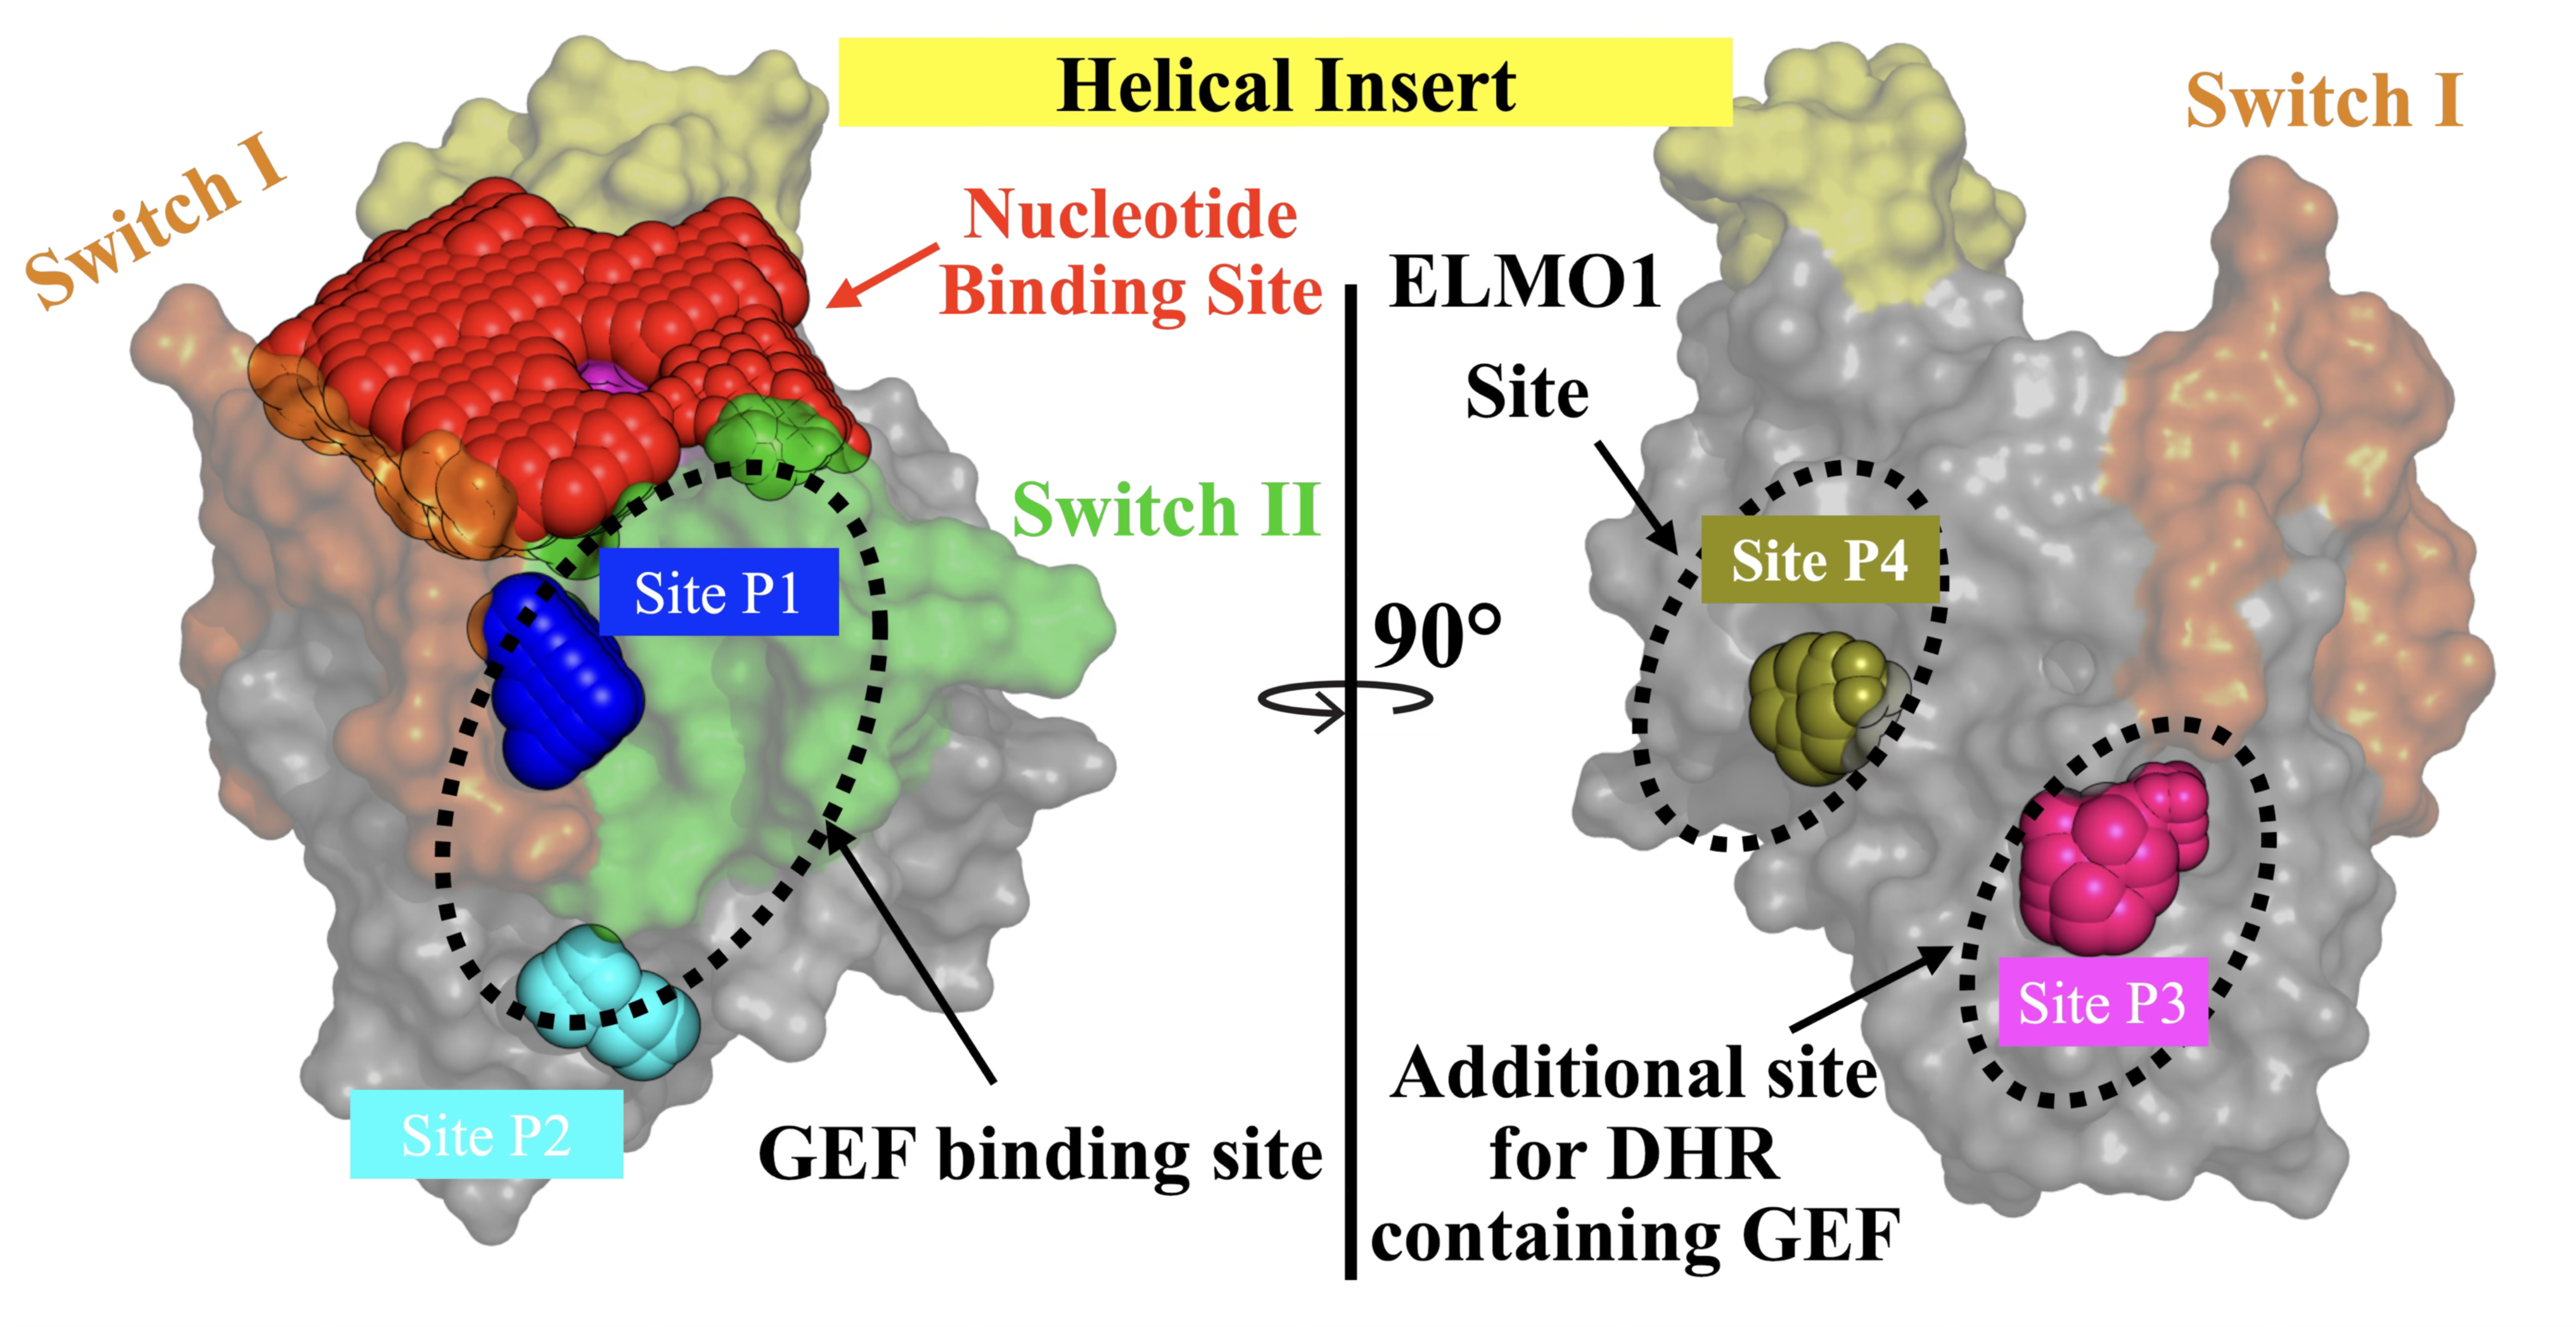
\includegraphics[width=\textwidth]{TOC.jpg}
\end{tocentry}

 \begin{abstract}
Rac1 (Ras-related C3 botulinum toxin substrate 1) serves as a molecular switch by hydrolysis of GTP \textcolor{red}{to} GDP. Due to the slow \textcolor{red}{rate of} hydrolysis of GTP and dissociation of GDP, Rac1 requires Guanine Exchange Factors (GEFs) and GTPase-activating proteins (GAPs) for \textcolor{red}{its} regulation. Despite being considered undruggable because of its small size and shallow surface, the binding of GAPs and GEFs \textcolor{red}{suggests existence} of transient binding pockets on Rac1. Using molecular dynamics simulations, we identified four such pockets: two serve as GEF binding sites, a third interacts with DHR domain-containing GEFs from the DOCK family, and the fourth binds the Engulfment and Cell Motility 1 (ELMO1) protein. To adequately sample the open states of these pockets, we used \textcolor{red}{cosolvent molecular probes} in MD simulations. \textcolor{red}{Principal component analysis of the cosolvent MD simulations helped us understand significant domain movements. We attempted to use this information to understand how these transient pockets open or close. Our work reveals transient pockets that GEF proteins could use, leading to new avenues for drug design opportunities.} 
\end{abstract}

\section{Introduction}
Small G proteins are a ubiquitous class of proteins that play pivotal roles in various cellular processes. Their functions include signal transduction, vesicle trafficking, cytoskeletal dynamics, and cell division. Ras GTPases regulate cell proliferation, differentiation, and survival. Rho GTPases govern cytoskeletal dynamics and cell migration.  These proteins possess conserved domains across several families; they are made up of six $\beta$-sheets surrounded by \textcolor{red}{five} $\alpha$-helices. All domains are conserved such that they carry a guanine nucleotide binding site to recognise the guanine base, \textcolor{red}{and the phosphate groups and magnesium ion}\cite{toma2019structural, cherfils2013regulation}. Two switch regions, switch I (SI) and switch II (SII), regulate the traffic to \textcolor{red}{this nucleotide binding site}. Their activity is regulated through a molecular switch mechanism by guanine nucleotide exchange factors (GEFs), GTPase-activating proteins (GAPs), and guanine nucleotide dissociation inhibitors (GDIs)\cite{cherfils2013regulation}. The mechanism cycles between OFF (GDP-bound inactive) and ON (GTP-bound active) states. This switching mechanism controls various processes like cell growth and differentiation to vesicular and nuclear transport\cite{cherfils2013regulation, loirand2013small}. It is also well established that small G proteins alone cannot \textcolor{red}{efficiently} hydrolyse GTP. Therefore,  \textcolor{red}{GEFs and GAPs assist in the catalytic function, and thus, the switching mechanism}. They control the dynamics of the switch regions that facilitate either the hydrolysis of GTP or the dissociation of GDP. GDP:Mg$^{2+}$ dissociates very slowly, and therefore, \textcolor{red}{GEFs function as exchange facilitatorm, the catalyses GDP dissociation}. \textcolor{red}{One of the accepted mechanisms by which GEFs expedite dissociation of GDP is by electrostatic repulsion of the magnesium ion that forms a strong interaction with small G proteins and phosphate groups of GDP. The loss of magnesium ion weakens the affinity of GDP, and thus dissociates}. \textcolor{red}{An alternate mechanism suggests that some GEFs can rearrange the switch I or II conformations to weaken GDP's affinity, thus catalysing its dissociation}.  GEFs are also known to enable GDP dissociation by combining the two mechanisms.\cite{cherfils1999gefs, cherfils2014gefs}. \textcolor{red}{GAPs are found to stabilise the transition state for GTP:Mg$^{2+}$ bound small G proteins, which catalyses the hydrolysis of the $\gamma$-phosphate group from GTP}. Taken together, the switching mechanism can be seen as GEFs assist in the activation of small G proteins, while GAPs assist in GTP hydrolysis. Following GTP hydrolysis, the inactive small G proteins prevent further signal transduction\cite{bos2007gefs}. 

In some classes of small G proteins, the active and inactive states are conjugated with small G proteins being shuttled between the cell membrane and cytosol. Such small G proteins undergo post-translational modifications to carry long-chain fatty acids at their C-terminal to assist bilayer insertion. GDIs\cite{dermardirossian2005gdis, maruta1998gtpase} sequester the lipid component to prevent membrane insertion of small G proteins. This coordinated action of small G proteins, GEFs, GAPs, and GDIs is essential for various cellular processes. Dysregulation of any of these components lead to pathologies such as cancer, neurodegeneration, and inflammatory disorders. For instance, mutations in Ras and its regulators are implicated in oncogenesis, highlighting the therapeutic potential of targeting small G protein signalling pathways\cite{cherfils2013regulation}. Such mutations (Q61L, Y72C, oncogenic P29S and Q61R, and negative T17N) are known to disrupt the equilibrium between the active and inactive states of small G protein\cite{rac1muts}. It has been observed that mutations either enhance the affinity of GEFs or GAPs that trap the small G proteins either in an activated or an inactivated state. Small molecule inhibitors targeting small G protein activity or disruptors of GEF/GAP interactions\cite{gray2020targeting} are under development for cancer therapy. However, there are several challenges in targeting small G protein and/or their GAP/GEF complexes. Targeting the guanine binding site is challenging owing to the large intracellular concentration of GTP and high affinity\cite{traut1994physiological}. In such cases, finding alternate sites can avoid such competition with endogenous substrates. GTPase hyper-activation or inactivation can be corrected by disrupting the protein-protein interaction (PPI) between small G protein and GEFs/GAPs by targeting the regulatory protein docking sites.   

\textcolor{red}{Amongst the small G proteins}, Rac1 plays a crucial role in regulating cellular processes owing to its switching mechanism that recruits several other proteins upstream and downstream. PREX1, TIAM1, VAV1 and DOCK2 are Rac1-specific GEFs that regulate many cellular processes and, therefore, are implicated in Rac-dependent pathologies such as asthma and cancer.  Structurally, PREX1, TIAM1 and VAV1 are DH/PH domain-containing proteins, while DOCK2 belongs to the family that contains the DHR domain. \textcolor{red}{The DH (Dbl homology) domain is an all-helical catalytic module that interacts with the switch I and II regions of GTPases to facilitate nucleotide exchange. The adjacent PH (Pleckstrin homology) domain regulates activity by promoting membrane localization through phosphoinositide binding and stabilizing the DH–GTPase complex\cite{prex1pdb,tiam1pdb,vav1pdb}.  The DHR-1 domain of DOCK family guanine nucleotide exchange factors\cite{dock2pdb} functions as a phosphoinositide-binding module that mediates membrane localization. It binds phosphatidylinositol-3,4,5-trisphosphate and phosphatidylinositol-4,5-bisphosphate, recruiting the DOCK–ELMO complex to phosphoinositide-enriched regions of the plasma membrane, particularly at the leading edge of migrating cells. This positioning enables spatially restricted activation of GTPases by the catalytic DHR-2 domain. Consequently, DHR-1 operates as a coincidence detector linking membrane lipid signals to GTPase activation. Mutations that disrupt phospholipid binding impair DOCK-dependent cell migration and polarization despite intact catalytic activity.}

Irrespective of their structural diversity, GEFs interact with the switch I and/or II region residues.  Since the nucleotide-binding site is well conserved among the small G protein family, this poses a significant challenge to selectively target Rac1 by targeting the orthosteric site. Furthermore, the molar concentration with picomolar binding affinity of GTP makes it more difficult for small molecules to competitively inhibit Rac1. The binding of GEFs with Rac1 shows the possibility of alternative binding sites that transiently open to allow this protein-protein interaction, opening a way for allosteric modulation. Therefore, the switching mechanism offers a conformational landscape that must be studied in detail that may lead to alternate binding sites on the Rac1 surface. Therefore, we embarked to understand the complete dynamical landscape of Rac1 protein bound to either nucleotides (GDP or GTP) or GEFs (PREX1, TIAM1, VAV1 or DOCK2).  \textcolor{red}{We tracked the formation of alternate binding pockets in its nucleotide-bound conformation and bound with its partners (holo). Following molecular dynamics simulations, we identified and measured the pocket volume changes for the newly identified transient pockets. We also monitored the effect of GEFs and nucleotide binding on the changes in the pocket volume. Lastly, using Pearson's correlation coefficient, we evaluated the possibility of correlation between changes in all four transient pockets among each other and the nucleotide binding site. Our study reveals cryptic pockets opening new possibilities for drug design.}

\section{Methods}\label{methods}
\subsection{Preparation of systems for molecular dynamics simulation} 
The coordinates for all complexes were retrieved from the Protein Data Bank (PDB); the PDB entries used in this study are listed in \textbf{Table \ref{tbl:pdbs}}. The X-ray structures were imported and processed in the UCSF Chimera v1.17 \cite{pettersen2004ucsf}. Any missing loops were built using Modeller \cite{fiser2003modeller} with UCSF Chimera v1.17 as the GUI \cite{yang2012ucsf, huang2014enhancing}. 

\begin{table}
  \caption{Rac1 conformations and binding partners used in this study}
  \label{tbl:pdbs}
  \begin{tabular}{c c c}
    \hline
   \textbf{PDB id} & \textbf{Rac1 Modulator/Ligand} & \textbf{Comments} \\
    \hline
    1HE1\cite{gappdb} &  GDP:Mg$^{2+}$ & Inactive Rac1 \\
    3TH5\cite{activeRac1}   & GTP:Mg$^{2+}$ & Active Rac1 \\
    4YON\cite{prex1pdb} & PREX1 (aa. 34-366) &  DBL family member \\
    1FOE\cite{tiam1pdb} & TIAM1 (aa. 1033-1406, mouse) &  DBL family member \\
    2VRW\cite{vav1pdb} & VAV1 (aa. 170-575, mouse) & DBL family member \\
    2YIN\cite{dock2pdb} & DOCK2 (aa. 1192-1622) & DOCK family member \\
    \hline
  \end{tabular}
\end{table}


\subsection{Generating AMBER-compatible parameters} 
 All systems were prepared for MD simulations with the Leap module in AMBERtools23. Protein atoms were atom-typed according to the AMBER14 (ff14SB) force field\cite{ff14sb}. Amber-compatible parameters for all nucleotides were obtained from the Manchester AMBER database\cite{meagher2003development}. For the VAV1 zinc finger region, the parameters of the Zinc atom, coordinating cysteines and histidine residues, the force field parameters were obtained from the ZAFF\cite{zaff} force field library.

\subsection{Molecular dynamics simulations} 
 All complexes were solvated with TIP3P\cite{tip3p} waters enclosed in a box with dimensions extending 10 \r{A} beyond any protein atom, and an appropriate number of neutralising ions were added to maintain the system's neutrality. The complexes were relaxed using three cycles of minimisation of 50000 steps each.  The first 5000 steps of minimisation adopted the steepest descent algorithm, and the remaining 45000 steps used the conjugate gradient algorithm. The cut-off for evaluating non-bonded interactions was placed at 8.0\r{A} for the minimisation phase. The first cycle of minimization was performed with  25 kcal/(mol.{\r{A}$^2$}) restraining force on the solute atoms, this force constant was reduced to 5 kcal/(mol.\r{A}$^2$) in the next cycle, and the final cycle was performed without any restraining forces on either the solute or the solvent atoms. The system was heated in 4 stages (see \textbf{Table \ref{SI-tbl:SI-Heating using NVT Ensemble}}) from 0 K to 300 K for 10 ns with  50 kcal/(mol.{\r{A}$^2$}) restraining force on the solute atoms using the Langevin dynamics, with a collisional frequency of  2 $ps^{-1}$.  The next step employed the NPT ensemble for density equilibration for another 2 cycles of 10 ns each, with the restraining force on the solute atoms gradually decreasing from 5 to 0 kcal/(mol.{\r{A}$^2$}). In the equilibration phase, the cut-off for evaluating non-bonded interactions was placed at 8 \r{A}. In the production phase of the MD simulations, all systems were simulated for 100 ns in triplicate, amounting to a 300 ns trajectory for each system.  The long-range electrostatic interactions were calculated using the Particle Mesh Ewald (PME) summation method\cite{pme}. The cut-off for evaluating non-bonded interactions was placed at 9.0 \r{A}  for the production phase. All the computations were done using the CUDA-enabled PMEMD code\cite{pmemd01, pmemd02, pmemd03} in AMBER22\cite{amber22, amber}.  
All simulations were performed with the SHAKE algorithm\cite{shake} to constrain bonds to hydrogen atoms, with the tolerance set to 0.00001 \r{A}.  A 2 fs integration time step was used to solve Newton's equations of motion.  For analysis, the conformations were saved every 100 ps, amounting to 1000 snapshots per trajectory (3000 per system). 


\subsection{Measuring the structural dynamics of Rac1} 
    Analysis of the MD trajectory was performed with the cpptraj\cite{cpptraj} module in AMBERTools23.  Before the analysis, all solvent atoms and neutralising ions were stripped off, and the protein conformations were aligned to their respective X-ray conformation.  The mass-weighted C$\alpha$ root-mean-square deviation (RMSD) for the protein was computed using the X-ray conformation as the reference. The root-mean-square fluctuations (RMSF) per residue for the backbone and side-chain atoms were computed to understand the domain-specific fluctuations.
    
\subsection{Identification and measurement of alternate pockets on Rac1} 
    POVME2 \cite{durrant2011povme, durrant2014povme} was employed for identifying various pockets on the Rac1. To be able to incorporate various experimental conformations of Rac1, we employed Rac1 with different binding partners (see \textbf{Table \ref{tbl:pdbs}}). To identify the pockets, the pocketID module on POVME2 was used on the aforementioned Rac1 structures. The parameters used for pocket identification are shown in \textbf{Table \ref{SI-tbl:SI-pocketParameters}}. Following the pocket identification, we monitored the pocket volume changes of these pockets throughout MD trajectories. It has been observed that the pocket might be a good candidate for druggability if its volume range was found to lie between 610--930 \r{A}$^3$\cite{perot2010druggable, nayal2006nature, an2005pocketome}.

\subsection{MD simulations with cosolvent Molecular probes} 
MD simulations with \textcolor{red}{cosolvent molecular probes} are very useful to accelerate pocket opening or to keep the transient pockets open for a longer period in MD simulations to better understand pocket characteristics. We identified transient pockets in response to GEF binding, which were otherwise not observed or very hard to locate. To ensure that these transient pockets can remain open sufficiently long to be druggable, we used cosolvent MD simulations. For this purpose, we used 1M concentration of isopropanol, phenol and toluene. The choice of these \textcolor{red}{cosolvent molecular probes} mimics drug-like fragments with decreasing water solubility. In this case isopropanol (logP = 0.05) $>$ phenol (logP = 1.39)  $>$ toluene (logP = 2.56). The simulation box with Rac1 protein (PDB: 3TH5, GTP and Magnesium ions were deleted) and 0.15M of NaCl was prepared using packmol \cite{martinez2009packmol}. \textcolor{red}{The number of cosolvent molecular probes was such that final simulations consists of 10\% concentration.} The protocol for MD simulations is the same as mentioned above. GAFF2 parameters were assigned to the organic solvents. For cosolvent MD simulations, we performed triplicate MD simulations for 1 \text{$\mu$s},  amounting to a total sampling time of 3 \text{$\mu$s} per solvent system. For the baseline calculations, we also prepared two systems without adding cosolvents.  One is the RAC1 complexed with GTP and Magnesium ions, which mimics an active-like conformation of RAC1. The apo system was created by deleting GTP and Magnesium ions from the active site system described previously. These systems would enable us to understand if any of the transient pockets can spontaneously open without the influence of the cosolvents and any ligand in the nucleotide pocket. \textcolor{red}{The probe density around the transient sites was computed using the radial distribution function ($g(r)$) as the function of distance. To evaluate the solvent accessible surface area (SASA) of the transient pockets, a 1.4 \r{A} probe atom. The SASA was computed on the residues that formed each of the transient site in cpptraj module of AMBERTools23. the The Pearson's correlation coefficient between the fluctuation observed in pocket volumes for each of the transient site was computed using pandas module in python3.}

\subsection{Principal component analysis of Rac1 protein following cosolvent MD}
\textcolor{red}{To understand the effect of \textcolor{red}{cosolvent molecular probes} on the Rac1, we extracted the essential dynamics using Principal Component Analysis (PCA) projected on the starting conformation used as the reference coordinate frame}. The Variance-Covariance matrix for C$\alpha$ atoms was extracted in the bio3D package\cite{bio3d} module in R Studio. We extracted and analysed four principal components; however, the first principal component with the largest eigenvalue was used to understand the essential dynamics in the Rac1 protein. The scree plot for each system is given in the supplementary \textbf{Figure \ref{SI-fig:SI_screeplot}}.

\subsection{\color{red}{Identifying the GEF binding hotspots on Rac1 surface using residue decomposition MMGBSA}} 

\textcolor{red}{To indentify the residues on Rac1 surface that interact with various GEF residues, we employed the residuewise decomposition of the binding enthalpy shown in the equation (Eq-\ref{eq:free-energy}) on the conformations saved from the MD simulations using the MMPBSA module\cite{mmpbsa} available in AMBERTools23;}

\begin{equation} \label{eq:free-energy}
     \   {\Delta}G_{\text{GBSA}} = {\Delta}G_{\text{Complex}} - ( {\Delta}G_{\text{Receptor}} - {\Delta}G_{\text{Ligand}})
\end{equation}

\textcolor{red}{Where  ${\Delta}G_{\text{Complex}}, {\Delta}G_{\text{Receptor}}$ and $ {\Delta}G_{\text{Ligand}}$ are binding enthalpy contributions calculates using Generalised-Born Surface Area (GBSA) method for the complex, receptor and ligand components respectively. The interaction energy between the binding partners is computed in the gas phase using a molecular mechanics (MM) method, and the correction to account for the solvent effects is added using the MM/GBSA method. The internal dielectric constant for GBSA calculations was set to 1, and the solvent dielectric constant was fixed at 80. For computing the binding affinity using the MM/GBSA method, the OBC’s GB model\cite{igb5} $ (igb = 5) $ was used. The mbondi2 radii set was employed to define the PB radii for all solute atoms during the preparation of the topology and parameter files in the leap module in AMBERTools23. The ionic strength for GBSA calculations was maintained at 150 mM. All energy components, in an implicit solvent, were calculated using a large cut-off of 999 \r{A}. The surface area for the non-polar solvation term was computed using the linear combination of pairwise overlaps (LCPO) method\cite{lcpo}. To identify the critical amino acid residues that are critical for the protein-protein interactions between Rac1 and GEFs, we computed the per-residuewise decomposition of the binding affinity. This enabled use to estimate the contribution to GEF binding from the residues that form the transient sites.}

\section{Results and discussion}
Protein-protein interactions are central to biology. By coordinating an intricate network of proteins that are recruited and activated in a pathway to pass the signal to the nucleus to control the rate and amount of protein expression. Such networks are tightly regulated by molecular switches, mainly by small G proteins, which are activated in response to GTP binding and turned off upon GTP hydrolysis to GDP. For the next switch on step, GDP must dissociate, which allows for GTP binding. However, the binding affinity of GDP and GTP are very high and comparable; therefore, GDP dissociation is not spontaneous. Thus, the guanine exchange must be assisted by GEFs that are recruited depending on the pathway. The exchange factors serve a dual role of nucleotide exchange and recruiting proteins downstream in the signal pathway by activating a specific GEF-dependent network of proteins. \textcolor{red}{Therefore, we performed molecular dynamics simulations of Rac1 to investigate the influence of its binding to different GEFs, nucleotides, or in the \textit{apo} state. GEF binding paves the way to unlock different binding sites on the Rac1 surface that are not normally observed in the \textit{apo} state.} We further investigate whether such sites are amenable to small-molecule targeting by measuring the pocket volume changes over the course of MD trajectories. We also studied the structural changes that Rac1 undergoes during the opening of these alternate sites, and if there is any noticeable change in the nucleotide binding site that may affect the GTP association or GDP dissociation. 

\subsection{\textcolor{red}{GEF docking opens transient pockets}}

\begin{figure}[hbt!]
    \centering
    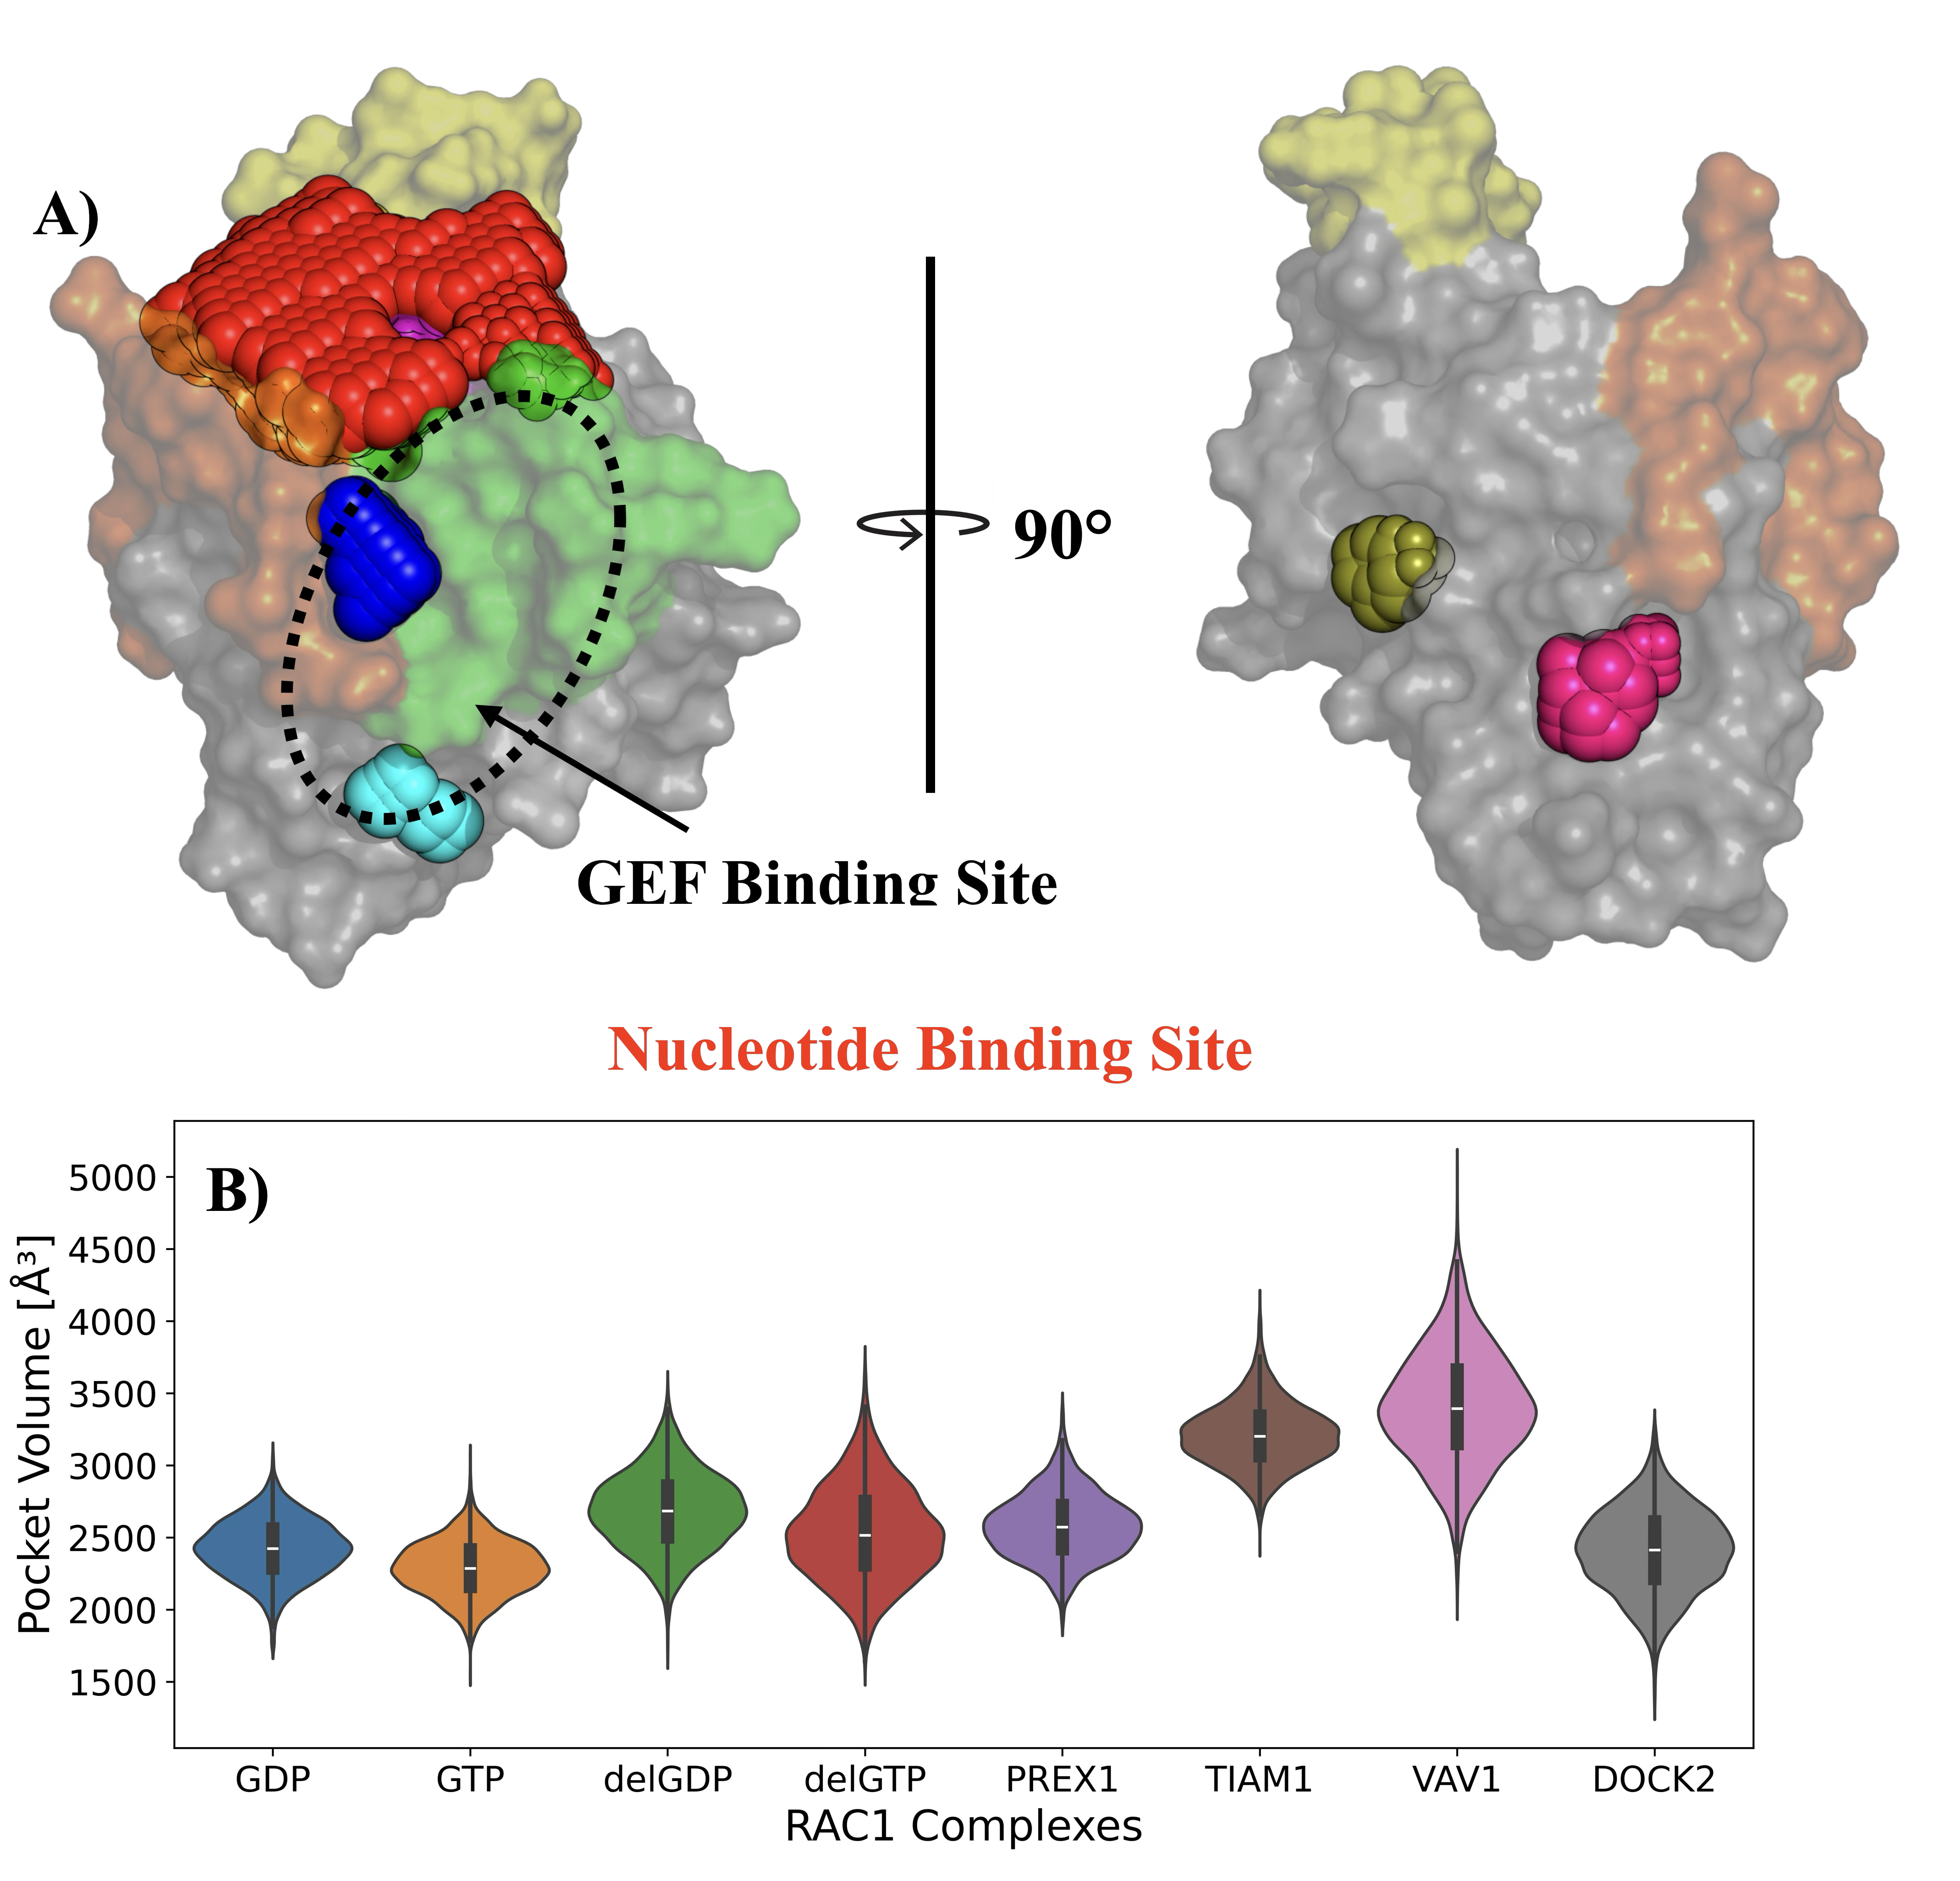
\includegraphics[width=1\textwidth]{Fig1.jpg}
    \caption{Identification and analysis of Rac1 pockets. \textbf{(A)} Rac1 surface with all possible binding pockets. The yellow-coloured region depicts the helical insert, which is peculiar to the Rho GTPase family. The orange-colored region depicts switch I, and the green coloured region is switch II. Red spheres occupy the nucleotide-binding site. Non-nucleotide binding pockets identified in this study are displayed in spheres representation. Pockets close to the nucleotide-binding site are in blue for site P1, in cyan for site P2. Pockets opposite to the nucleotide-binding site are in magenta for site P3, and asparagus for site P4. \textbf{(B)} The violin plot illustrates the distribution of the pocket volumes for each of the nucleotide-binding sites. The changes in the pocket volumes are monitored when Rac1 is complexed with either GEFs, GDP, GTP or in the \textit{apo}-states named as delGDP (GDP deleted from GDP-bound system), and delGTP (GDP deleted from GTP-bound system). \textcolor{red}{\textbf{(C)} The violin plot illustrates the distribution of the pocket volumes for the nucleotide-binding sites. The changes in the pocket volumes are monitored when Rac1 is simulated cosolvent molecular probes}. The amino acid numbering for Rac1 follows the Uniprot ID: P63000.}  
    \label{fig:pockets}
\end{figure}

We employed the POVME2\cite{durrant2014povme} tool to identify and measure the pocket volumes of new transient sites. \textcolor{red}{To futher validate the pockets identified by POVME2, we also employed Fpocket\cite{le2009fpocket} tool to characterise the pockets for its druggability score and hydrophobicity score.} By definition, transient or cryptic pockets are observed only in \textit{holo} proteins, while being undetectable in \textit{apo} proteins. We used various Rac1 structures bound to GEFs and nucleotides (\textbf{Table \ref{tbl:pdbs}}). To measure the pocket volumes over time, we simulated all Rac1 complexes (\textbf{Table \ref{tbl:pdbs}}). Before measuring the pocket volumes, all binding partners, including nucleotides, were deleted from the trajectory. In other words, the Rac1 conformation was allowed to evolve in the presence of the binding partners, which might allow the opening of the transient pockets. \textcolor{red}{Fpocket also identified the same number of pockets as did POVME2 (see \textbf{Table \ref{SI-tbl:SI-Fpocket}}).  We observed that according to Fpocket all the sites in question are poorly druggable. The pocket identification was performed using the X-ray conformations, in most enteries these transient pockets appear to be poorly formed.} \textcolor{red}{ Furthermore, to quickly estimate the hydrophobicity of the transient sites and to complement the predict by Fpocket, we measured the solvent-accessible solvent area for these site.  All the transient sites show SASA well above 200 \r{A}$^2$ except for Site P2 for GTP and delGTP systems, where it is significantly lower indicating the sites might have collapsed. (See \textbf{Supplementary Figures \ref{SI-fig:SI_SASA_100ns}}). Surprisingly, the SASA for Site P2 and P4 decrease significantly in presence of cosolvent molecular probes(See \textbf{Supplementary Figures \ref{SI-fig:SI_SASA_cosolv}})}.

We observed that the change in the nucleotide pocket volume was influenced by GEFs and the nucleotides. The pocket volume fluctuations remained under 3000 \r{A}$^3$ in the presence of GTP, and GDP (\textbf{Figure \ref{fig:pockets}B}) which indicates tight binding to nucloetides causing pocket volumes to shrink. Next, we monitored the changes in the pocket volumes by deleting the GTP and GDP to create \textit{apo}-like states called "delGTP" and "delGDP" respectively. This would enable us to understand the pocket dynamics in the absence of nucleotides, however, this is purely theoretical state since truly \textit{apo} state for Rac1 has never been isolated and studied experimentally.  We note a significant increase in the pocket volumes exceeding 3000 \r{A}$^3$ for both the \textit{apo}-like states. This marked increase in the pocket volumes in the \textit{apo}-like state can be attributed to an increased flexibility in the switch regions and the P-loop (\textbf{Figure \ref{fig:MD}B} and \textbf{supplementary Figure \ref{SI-fig:SI_RMSD_PL}}), which directly interacting with the nucleotides. A more noticeable difference in flexibility (\textbf{Figure \ref{fig:MD}B}) can be seen in the P-loop and the switch I loop (\textbf{supplementary Figure \ref{SI-fig:SI_RMSD_PL}} and \textbf{\ref{SI-fig:SI_RMSD_S1}}). 


\begin{figure}[hbt!]
    \centering
    \includegraphics[width=1\textwidth]{Fig_domain_RMSF.jpg}
    \caption{\color{red}{Rac1 domains and dynamics of each region. \textbf{(A)} Cartoon representation of human Rac1 (\textbf{PDB id:1HE1}). The P-loop region is depicted in magenta. The switch I region is depicted in orange, and the green coloured region is the switch II region. The helical region is shown in yellow colour. \textbf{(B)} Atomic fluctuations of all atoms measured as Root-Mean-Squared Fluctuations (RMSF) for the human Rac1 domain to compare the effect of nucleotide binding on the dynamics of various domains. \textbf{delGDP} and \textbf{delGTP} are systems created by deleting the nucleotides from the Rac1 binding pocket to create the corresponding \textit{apo} system. \textbf{(C)} Atomic fluctuations of all atoms  measured as Root-Mean-Squared Fluctuations (RMSF) for the human Rac1 domain to compare the effect of GEF binding on the dynamics of various domains. \textbf{(D)} Atomic fluctuations of all atoms  measured as Root-Mean-Squared Fluctuations (RMSF) for the human Rac1 domain to compare the effect of \textcolor{red}{cosolvent molecular probes} on the dynamics of various domains.}} 
    \label{fig:MD}
\end{figure}

The switch region conformation is also found to be reduced by GEF binding (\textbf{Figure \ref{fig:MD}C}), suggesting their role in controlling the nucleotide traffic by modulating the switching regions.  We tested this hypothesis by simulating a nucleotide-free and GEF-free form of Rac1 (delGDP and delGTP in \textbf{Figure \ref{fig:pockets}B}) and found that the pocket volume and fluctuations showed a tendency to increase, however, only marginally, as the volume was still under 4000 \r{A}$^3$. Next, we measured the pocket volume and the atomic fluctuations in the presence of GEFs in the nucleotide-free state.  The volume fluctuations appear to be higher than in the nucleotide-free state without GEFs. However, the volume changes showed significant changes among different GEFs. For example, PREX1 and DOCK2 showed volumes that are similar in magnitude to \textit{apo}-like states (delGDP and delGTP in \textbf{Figure \ref{fig:pockets}B}).  TIAM1 and VAV1 showed enlarged nucleotide pockets with volume above 4000 \r{A}$^3$. We hypothesise that such a difference in pocket volumes owing to different GEFs suggest that the X-ray structure has captured the Rac1-GEF complexes either just after GDP dissociation (PREX1 and DOCK2) or in a state that was pre-organised for GTP:Mg$^{2+}$ association (TIAM1 and VAV1). As we have already established that pocket volume changes in the nucleotide site can be attributed to the P-loop and switch region dynamics, it becomes apparent that GEFs interacting primarily with the switch region can control the nucleotide exchange (\textbf{Figure \ref{fig:MD}C}). The nucleotide-binding pocket is seen to enlarge with all GEFs, which could be a prerequisite for GDP dissociation. Perhaps an enlarged nucleotide site could facilitate association of GTP and Mg$^{2+}$. 

\begin{figure}[hbt!]
    \centering
    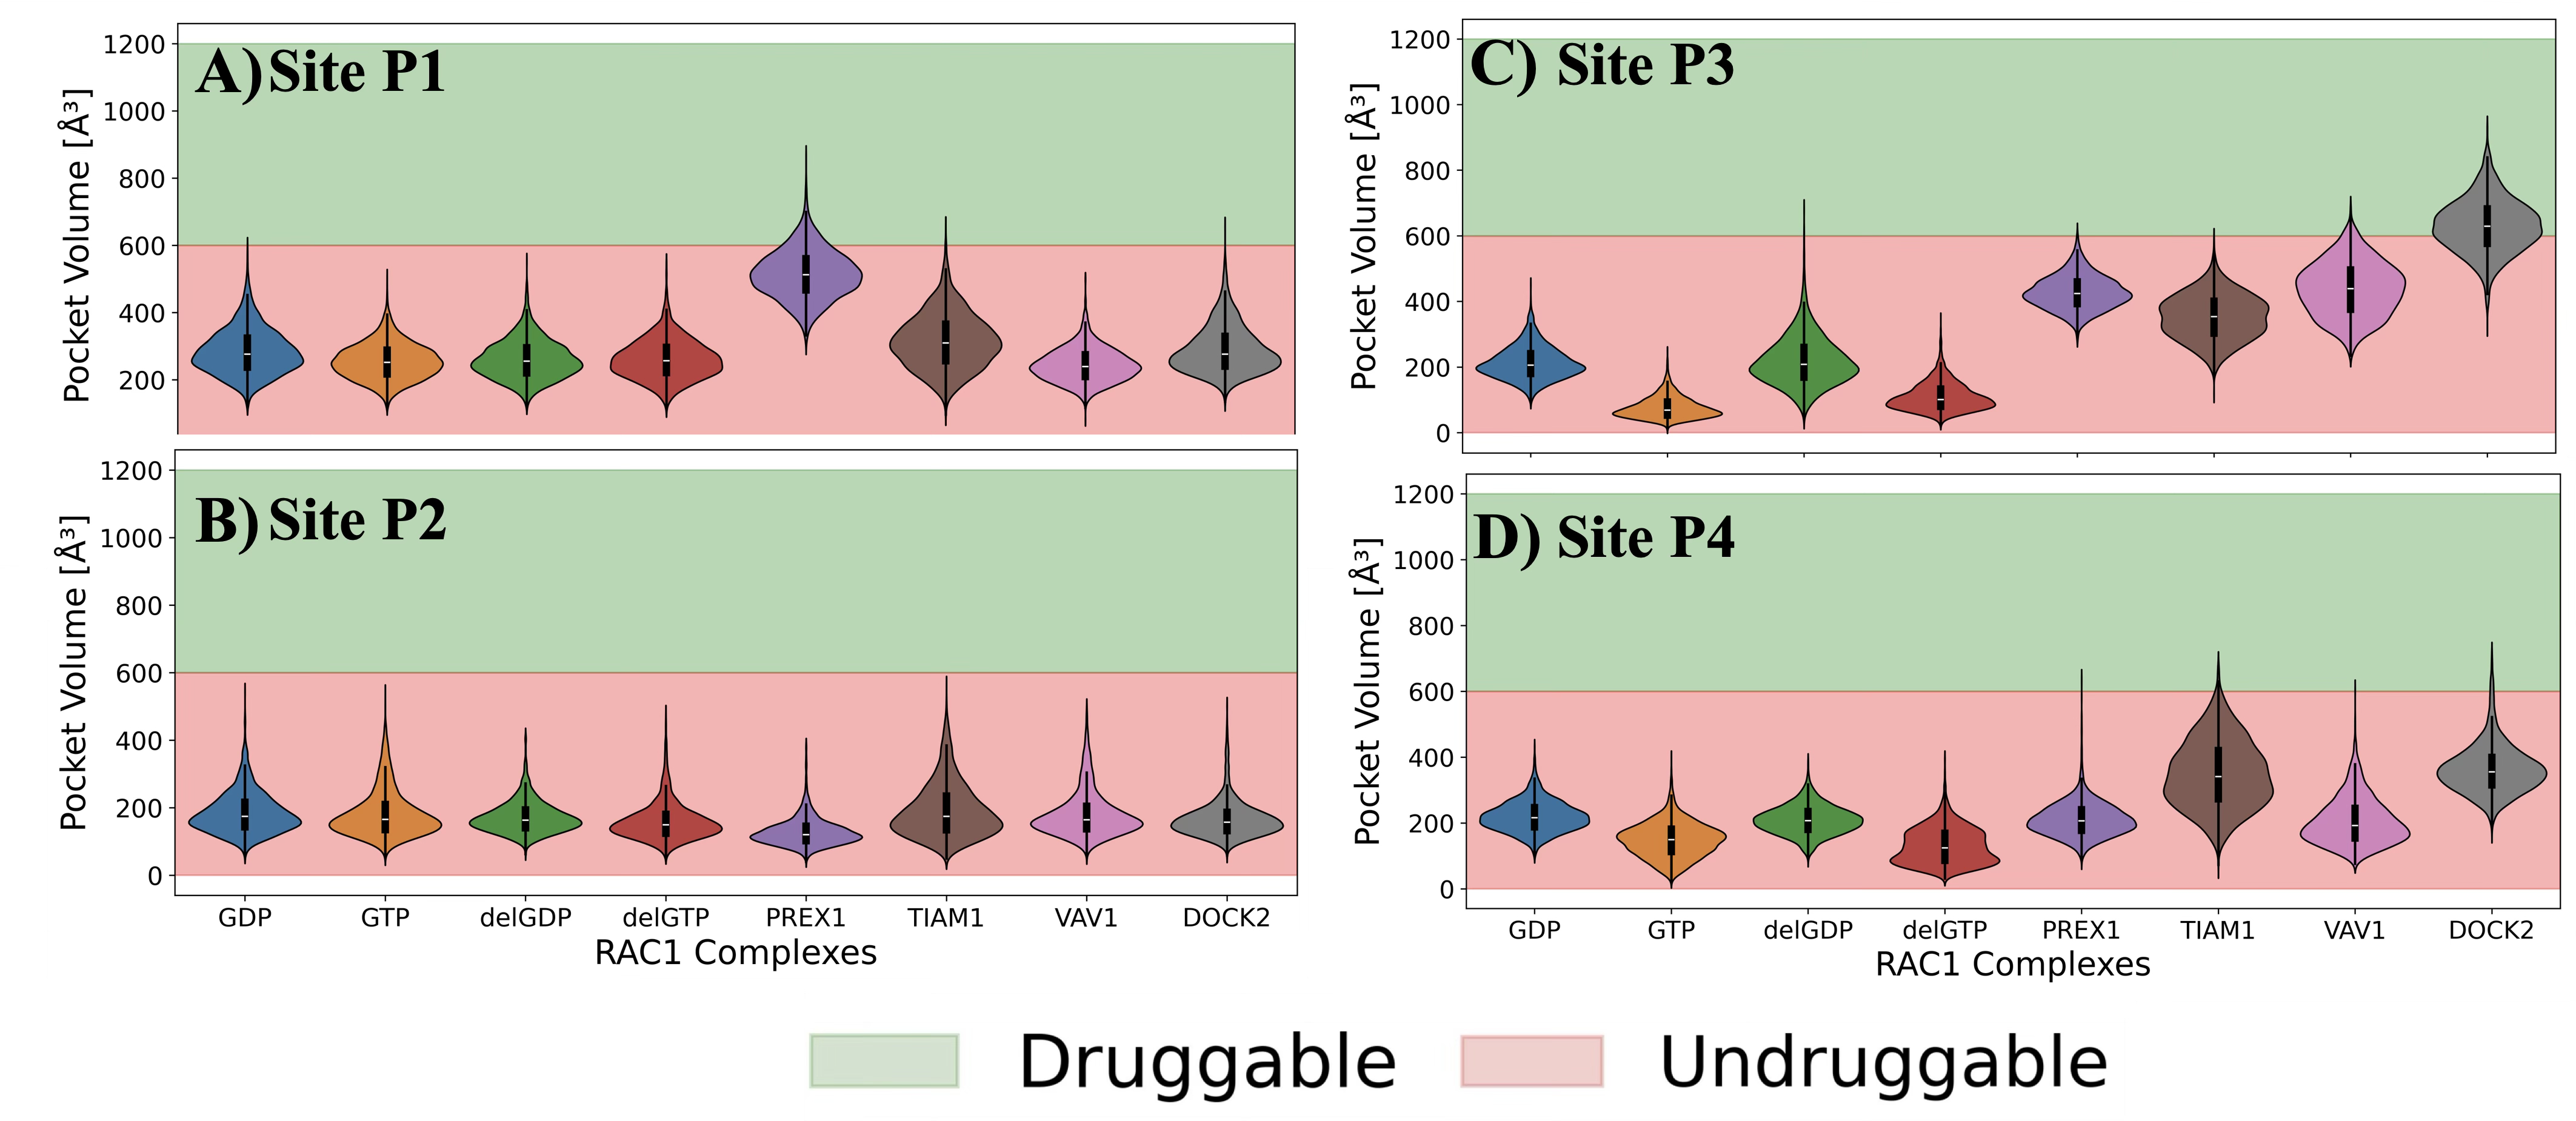
\includegraphics[width=1\textwidth]{Fig_transient_sites.jpg}
    \caption{Analysis of the four non-nucleotide binding pockets identified using POVME2. \textbf{(A)} Site P1 is located between switch regions I and II. \textbf{(B)} Site P2 is located at the bottom of the switch I and II loops at the N-terminal region. \textbf{(C)} \textcolor{red}{Site P3 is located at the beginning site of the switch I region.} \textbf{(D)} Site P4 is the only pocket that is not located close to switch I or II regions; however, this site appears to accommodate the ELMO1 protein that assists the DOCK family of GEFs in their function. The threshold value, beyond which a pocket may be considered amenable for small molecule binding, was set according to the following references\cite{perot2010druggable, nayal2006nature, an2005pocketome} and indicated by the dashed line.} 
    \label{fig:otherpockets}
\end{figure}

  \begin{table}
  \caption{Static Pockets volume computed using the X-ray conformation}
  \label{tbl:pocketID}
  \begin{tabular}{cccccc}
    \hline
   \textbf{Rac1 System}  & \textbf{Nucleotide Site}\textsuperscript{\emph{1}} & \textbf{Site P1}\textsuperscript{\emph{1}} & \textbf{Site P2}\textsuperscript{\emph{1}} & \textbf{Site P3}\textsuperscript{\emph{1}} & \textbf{Site P4}\textsuperscript{\emph{1}} \\
    \hline
    GTP & 2164 & 58 & 100 & 188 & 86\\
    delGTP & 2164 & 58 & 100 & 188 & 86 \\
    GDP & 2641 & 135 & 276 & 354 & 208 \\
    delGDP & 2641 & 135 & 276 & 354 & 208  \\
    PREX1 & 2694 & 399 & 171 & 518 &  335 \\
    TIAM1 & 2651 & 301 & 301 & 267 & 234  \\
    VAV1 & 3358 & 428 & 115 & 224 &  335 \\
    DOCK2 & 2327 & 658 & 268 & 221 &  99 \\
    \hline
  \end{tabular}
  
  \textsuperscript{\emph{1}}All pocket volumes reported in \r{A}$^3$.
\end{table}

We identified four transient pockets on the Rac1 surface that cannot be located with Rac1 structure alone. The sites P1 and P2 are located in the region lining the switch regions I and II. These sites form the binding site for the GEFs that perturb the switch regions, leading to the opening of these sites. Our pocket volume measurements indicate that the volumes are large enough to accommodate small-molecule binders (\textbf{Figure \ref{fig:otherpockets} and Table \ref{tbl:pocketID}}). In the absence of the GEFs, these sites are too small, and hence, not detected in GEF-free Rac1 (\textbf{Figure \ref{fig:pockets}A} and \textbf{supplementary Figure \ref{SI-fig:SI_P1_VOL}}).  
Sites P1 and P2 are present at a crucial location that modulates the dynamics of the switch regions. Thus, we hypothesise that one of the consequences of targeting these sites is that it could compete with GEF binding. Alternatively, the molecules occupying these sites could act as molecular glues that stabilise the Rac1-GEF complex, slowing the switching mechanism and thus, the nucleotide exchange. Both scenarios suggest that the modulation perturbs the GEF-mediated downstream signalling (\textbf{Figure \ref{fig:otherpockets}B} and \textbf{supplementary Figure \ref{SI-fig:SI_P2_VOL}}). We also acknowledge that one of the secondary effects of targeting site P1 and P2 opens up a possibility to occlude GTP binding, albeit non-competitively. According to one of the accepted mechanisms of nucleotide exchange\cite{cherfils2013regulation}, GTP binding weakens the GEF binding, which eventually dissociates. By preventing or decreasing the rate of GEF dissociation, GTP binding could be prevented or slowed down. Thereby prolonging the nucleotide-free state and preventing the downstream signalling. Site P2 is located below Site P1, and also found to marginal increase in the pocket volume in the presence of GEFs (\textbf{Figure \ref{fig:otherpockets}B}). We propose that, owing to the proximity, this could serve as an extension for molecules binding to Site P1 (\textbf{Figure\ref{fig:pockets}A} and \textbf{supplementary Figures \ref{SI-fig:SI_combinedpockets}A and \ref{SI-fig:SI_combinedpockets}B}).

Away from the GEF binding site are located sites P3 and P4 (\textbf{Figure \ref{fig:pockets}A}). Site P3 is located towards the N-terminal side of the switch I region. From the X-ray crystallographic information, residues lining the site P3 are known to interact more specifically with DHR-containing GEFs belonging to the DOCK family\cite{DOCK5_EMLO1, dock2pdb}. Targetting site P3 could possibly interfer with GEF binding especially from DOCK family. The ELMO1 protein that facilitates the binding of the DOCK family of GEFs is known to interact with residues that form the site P4\cite{DOCK5_EMLO1}. Taken together, we hypothesise that modulation of site P3 and P4 could specifically target and modulate the downstream signalling involving the DOCK family of GEFs. Pocket volume changes in site P3 and P4 show marked increase when bound to DOCK2 ((\textbf{Figure \ref{fig:otherpockets}C and \ref{fig:otherpockets}D} and \textbf{supplementary Figures \ref{SI-fig:SI_P3_VOL} and \ref{SI-fig:SI_P4_VOL}})) 

Lastly, we sought to find out if there exists any correlation in the pocket volume fluctuations among all the pockets. We used Pearson's correlation cofficient, and observed only marginal or neglible correlations (\textbf{Figures \ref{SI-fig:SI_CORRNUC}} and \textbf{\ref{SI-fig:SI_CORRGEF}}). However,in the delGDP system shows a moderately positive correlation between Site P2 and Site P3. However, we could not ascertain any noticeable atomic motions that explains this correlation for this isolated observation. In general, there exists negligible correlation in the pocket volume fluctuations. 


\subsection{\color{red}{Accelerating the pocket opening using cosolvent molecular probes}}

\begin{figure}[hbt!]
    \centering
    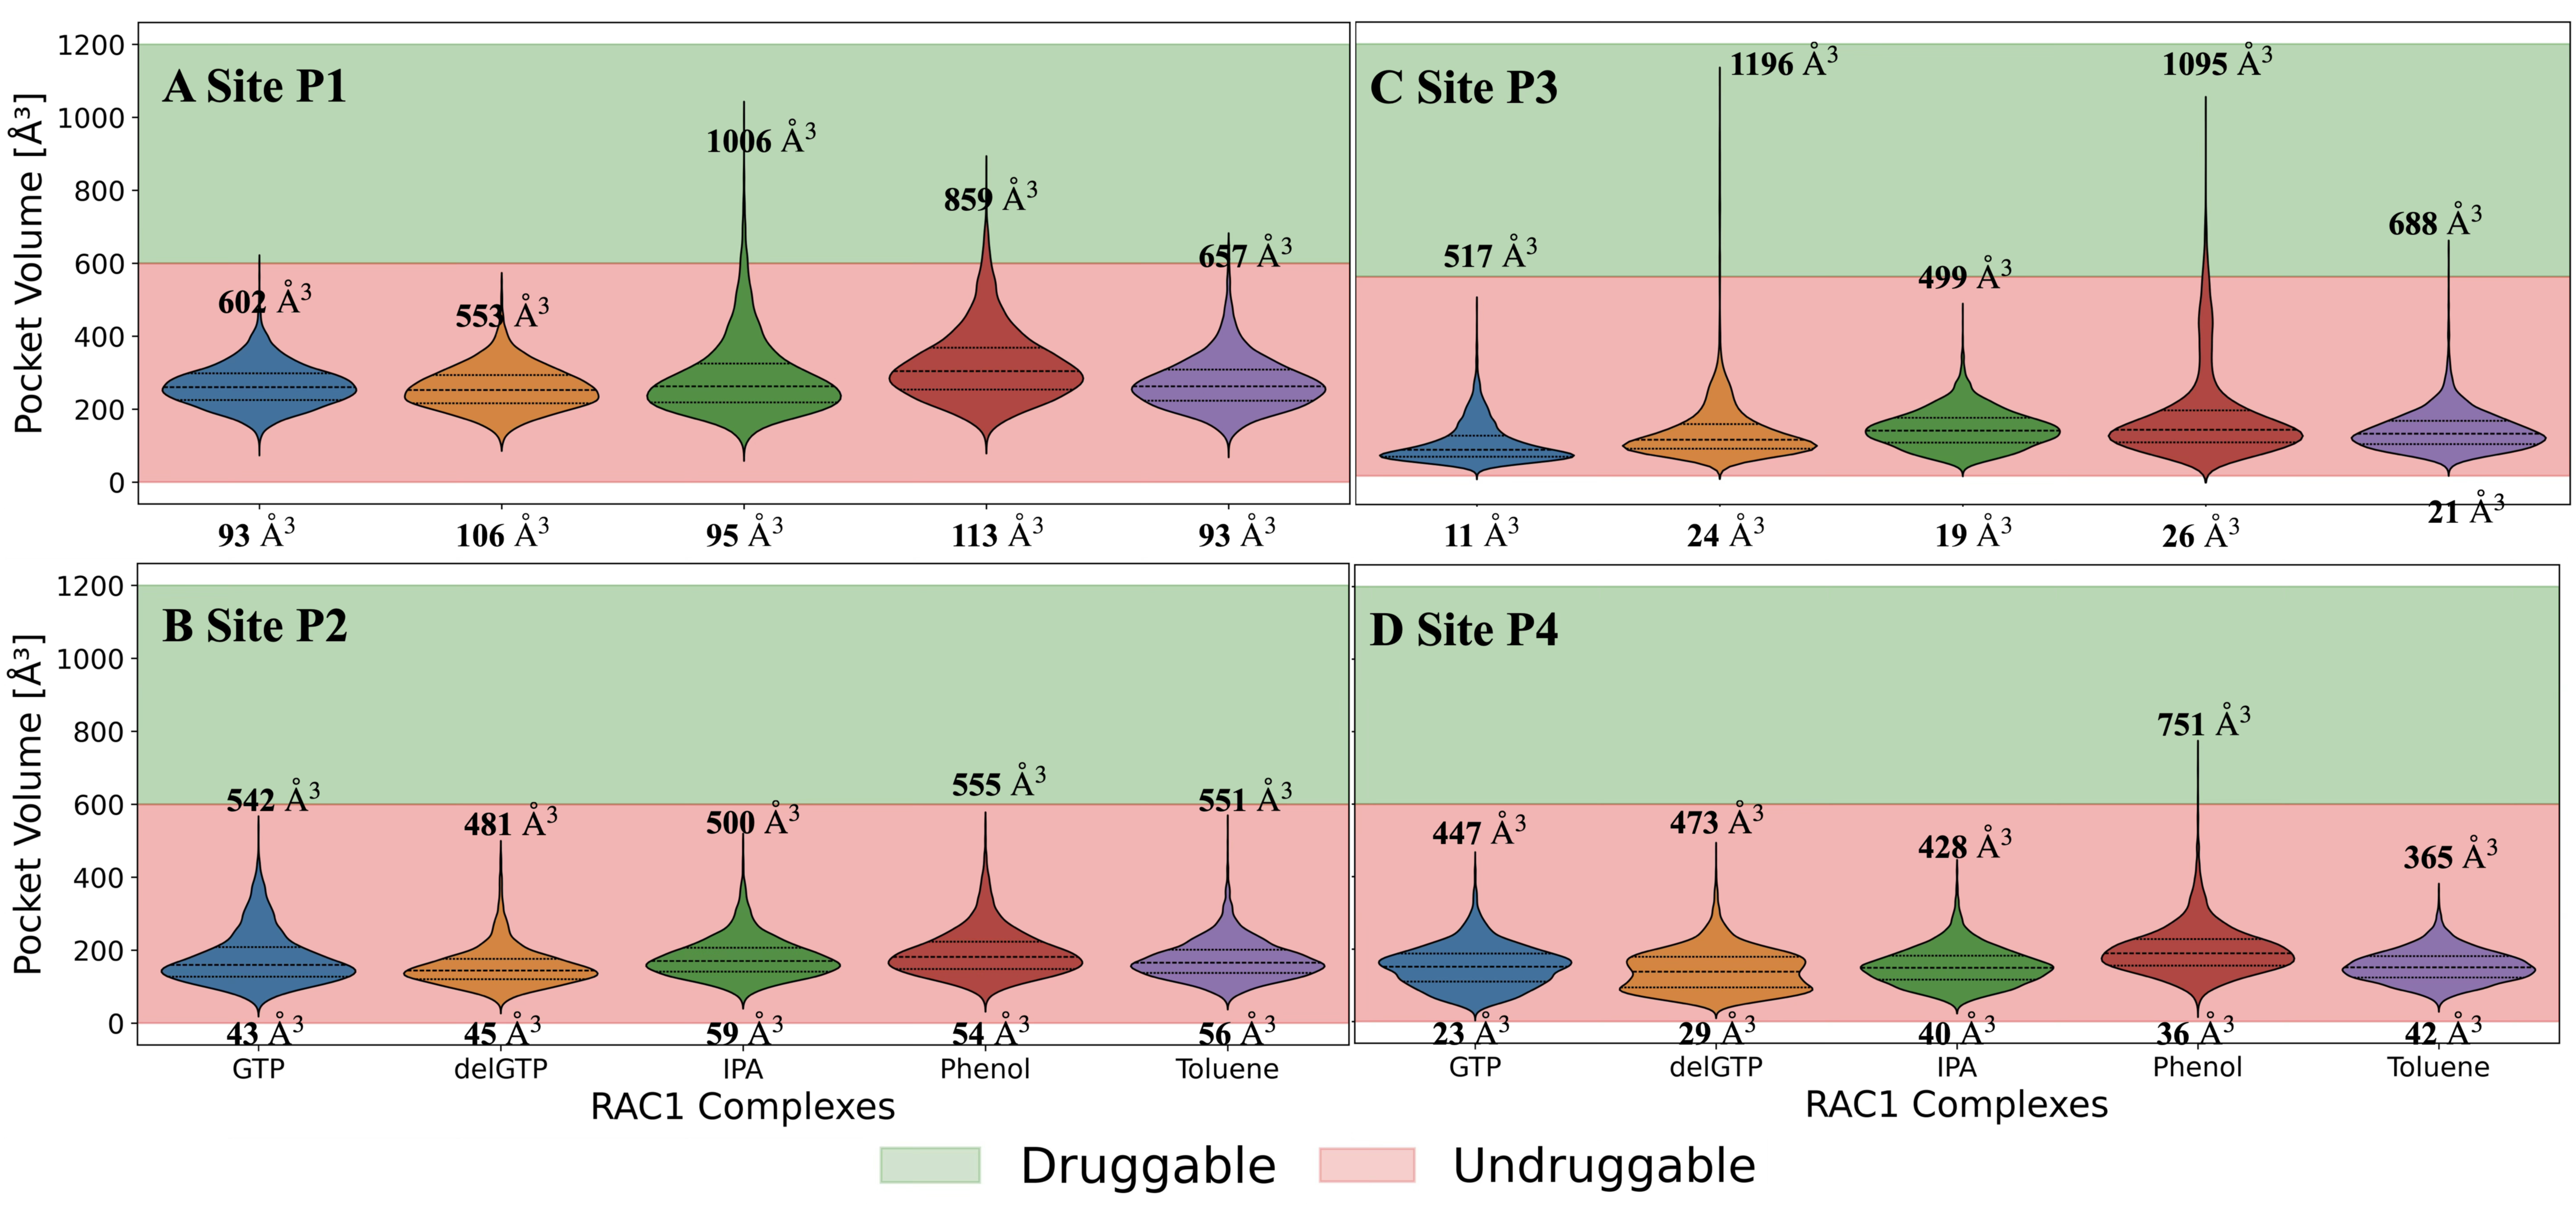
\includegraphics[width=1\textwidth]{Fig_transient_sites_cosolvents.jpg}
    \caption{Pocket volume measurements following cosolvent MD simulations for \textbf{(A)} Site P1, \textbf{(B)} site P2, \textbf{(C)} site P3, and \textbf{(D)} site P4.  The threshold value, beyond which a pocket may be considered amenable for small molecule binding, was set according to the following references\cite{perot2010druggable, nayal2006nature, an2005pocketome} and indicated by the dashed line.}
    \label{fig:cosol}
\end{figure}

In general, transient pockets open in response to ligand binding, suggesting an induced fit mechanism that triggers opening of the pocket(s). However, in the absence of any known ligands, \textcolor{red}{cosolvent molecular probes} that structurally resemble drug-like fragments are used as chemical probes to open such transient sites. We used three common \textcolor{red}{cosolvent molecular probes} with varying hydrophobicities to assess their ability to open the transient sites in the absence of GEFs. This coould also test the ability of such sites to be targeted by small molecules. The PBD entry with accession number \emph{3TH5} is the only X-ray crystal structure that is crystallised in the active-like conformation bound to GTP analogue, Guanylyl imidodiphosphate (GNP), without any regulatory protein. Rac1 conformation in this case shows that all GEF-induced pockets are in the undruggable state, evident by their small pocket volumes. We performed \textcolor{red}{triplicate} microsecond timescale MD simulations to check the effectiveness of the chemical probes to open the transient pockets through the induced-fit mechanism. We observe that at three sites, P1, P3, and P4, the pocket volumes cross the threshold value(\textbf{Figure \ref{fig:cosol}}).  \textcolor{red}{Therefore, suggesting that these pockets can open in response small molecular probes. However, we did not observe the systems, GTP and delGTP, simulate without cosolvent molecular probes sampled the conformations in which the pocket volumes crossed the threshold value, except for site P3 in delGTP(\textbf{Figure \ref{fig:cosol}C}). This could suggest that pockets are cryptic in nature, however, also acknowlegde the fact that this could also be a limitation of the sampling time scale used in the work, the spontaneous opening of the pockets may be observed well beyond the microsecond time scale.  Nevertheless, the current observation suggest that the cosolvent molecular probe can expedite the opening of the pockets.}

In the case of site P1, the pocket volume for the reference systems (GTP and delGTP) largely remains below the threshold for druggability. The chemical probes, isopropanol and phenol, can open this site significantly larger than the reference system, attaining a maximum volume of 1006\r{A}$^3$ and  859\r{A}$^3$ respectively (\textbf{Figure \ref{fig:cosol}A}). While using a completely hydrophobic probe, toluene, the pocket volume increased only marginally (maximum volume measured is 657\r{A}$^3$). This can be attributed to the phase separation observed for toluene molecules due to its high hydrophobicity, which leads to practically insoluble in water. To prevent such phase separation, it is recommended to use an intermolecular repulsive potential applied to probe molecules\cite{cosolvkit}. For site P2, none of the chemical probes were able to increase the pocket volume above the threshold value (\textbf{Figure \ref{fig:cosol}B}). Upon careful observation, we note that the site P2 is lined by $\beta$-sheets, which form the majority of the site. This leads to a rather flat pocket lined by rigid secondary structural elements, leaving little scope for movements that could increase the pocket volume. However, we expect this site, P2, to serve as a subpocket for site P1 binders that can be expanded to site P2 to increase the binding affinity. 

Site P3 appears to be open spontaneously in \textit{apo}-like (delGTP) with a maximum volume measured is 1196\r{A}$^3$ (\textbf{Figure \ref{fig:cosol}C}). While the pocket volume remained beyond the threshold for GTP-bound Rac1, and with IPA. However, phenol and toluene could push the maximum volume beyond the threshold, wherein with phenol the maximum volume measured was 1095\r{A}$^3$, which is similar magnitude to delGTP. The residues that make up site P3 appear to be mainly aromatic and aliphatic, which makes this pocket a hydrophobic patch (\textbf{Figure \ref{fig:pockets}A}). Therefore, the hydrophilic molecular probe, IPA, was unable to sample the open state of the pocket, whereas the hydrophobic probes like phenol and toluene did sample the open state of the pocket, wherein the pocket volume measures crossed the druggability threshold. Site P4 appears to be the smallest among the four transient pockets identified in this work. We observed that only in the phenol system the pocket volume crossed the druggability threshold with a maximum volume of 751\r{A}$^3$ (\textbf{Figure \ref{fig:cosol}D}). Upon closer inspection of the binding site residues, we observe a good balance of hydrophobic and charged residues, owing to which phenol, which comprises a hydrophobic ring with a hydrophilic hydroxy group, was able to open to the pocket beyond the threshold value. 

We note that three out of four pockets are indeed transient in nature, which can be open in an induced-fit manner. This is exemplified by the GEF-binding and the \textcolor{red}{cosolvent molecular probes}. We did choose the GTP-bound conformation of the Rac1 protein in which all four pockets reported the pocket volumes below the threshold value (\textbf{Figure \ref{fig:otherpockets}}). This way we could assure that in the starting conformation all pockets could be labelled as practically undruggable, giving an unbiased starting point to test the ability of the \textcolor{red}{cosolvent molecular probes} to open the pockets. 

\textcolor{red}{The radial distribution functions (supplmentary \textbf{figure \ref {SI-fig:SI_RDF}}) suggests the probability density $g(r)$ of three cosolvent molecular probes around the transient sites on the Rac1 surface. At site P1, the RDF profile shows a high probability of toluene molecules, with a peak exceeding $g(r) \approx 3$ around $\sim15$--$20$ \r{A}. Phenol exhibits moderate probability ($g(r)\sim1.5$--$2$), while IPA remains weakly populated. This suggests that site P1 is a hydrophobic hotspot, exemplified by preference towards toluene and phenol over a hydrophilic IPA. A similar trend can be observed at site P2, although the density of the probes is less than at site P1.  Toluene again shows the highest RDF peak ($\sim2$--$2.3$), followed by phenol and then IPA. In contrast, site P3 displays a different tendency, wherein phenol and toluene show comparable RDF maxima, with phenol shows slightly enhanced density at shorter radial distances. This shift indicates that polar aromatic groups could occupy this site. An increased phenol density at shorter distances suggests the presence of residues capable of forming hydrogen bonds or polar contacts in addition to hydrophobic interactions. At site P4, density of toluene is the largest RDF peak ($\sim2.2$). However, we are aware that toluene also shows a maximum possibility of aggregation in the absence of any repulsive potentials used during the simulations.}

\subsection{\color{red}{Is the switch region dynamics responsible for formation of cryptic pockets?}}

\begin{figure}[hbt!]
    \centering
    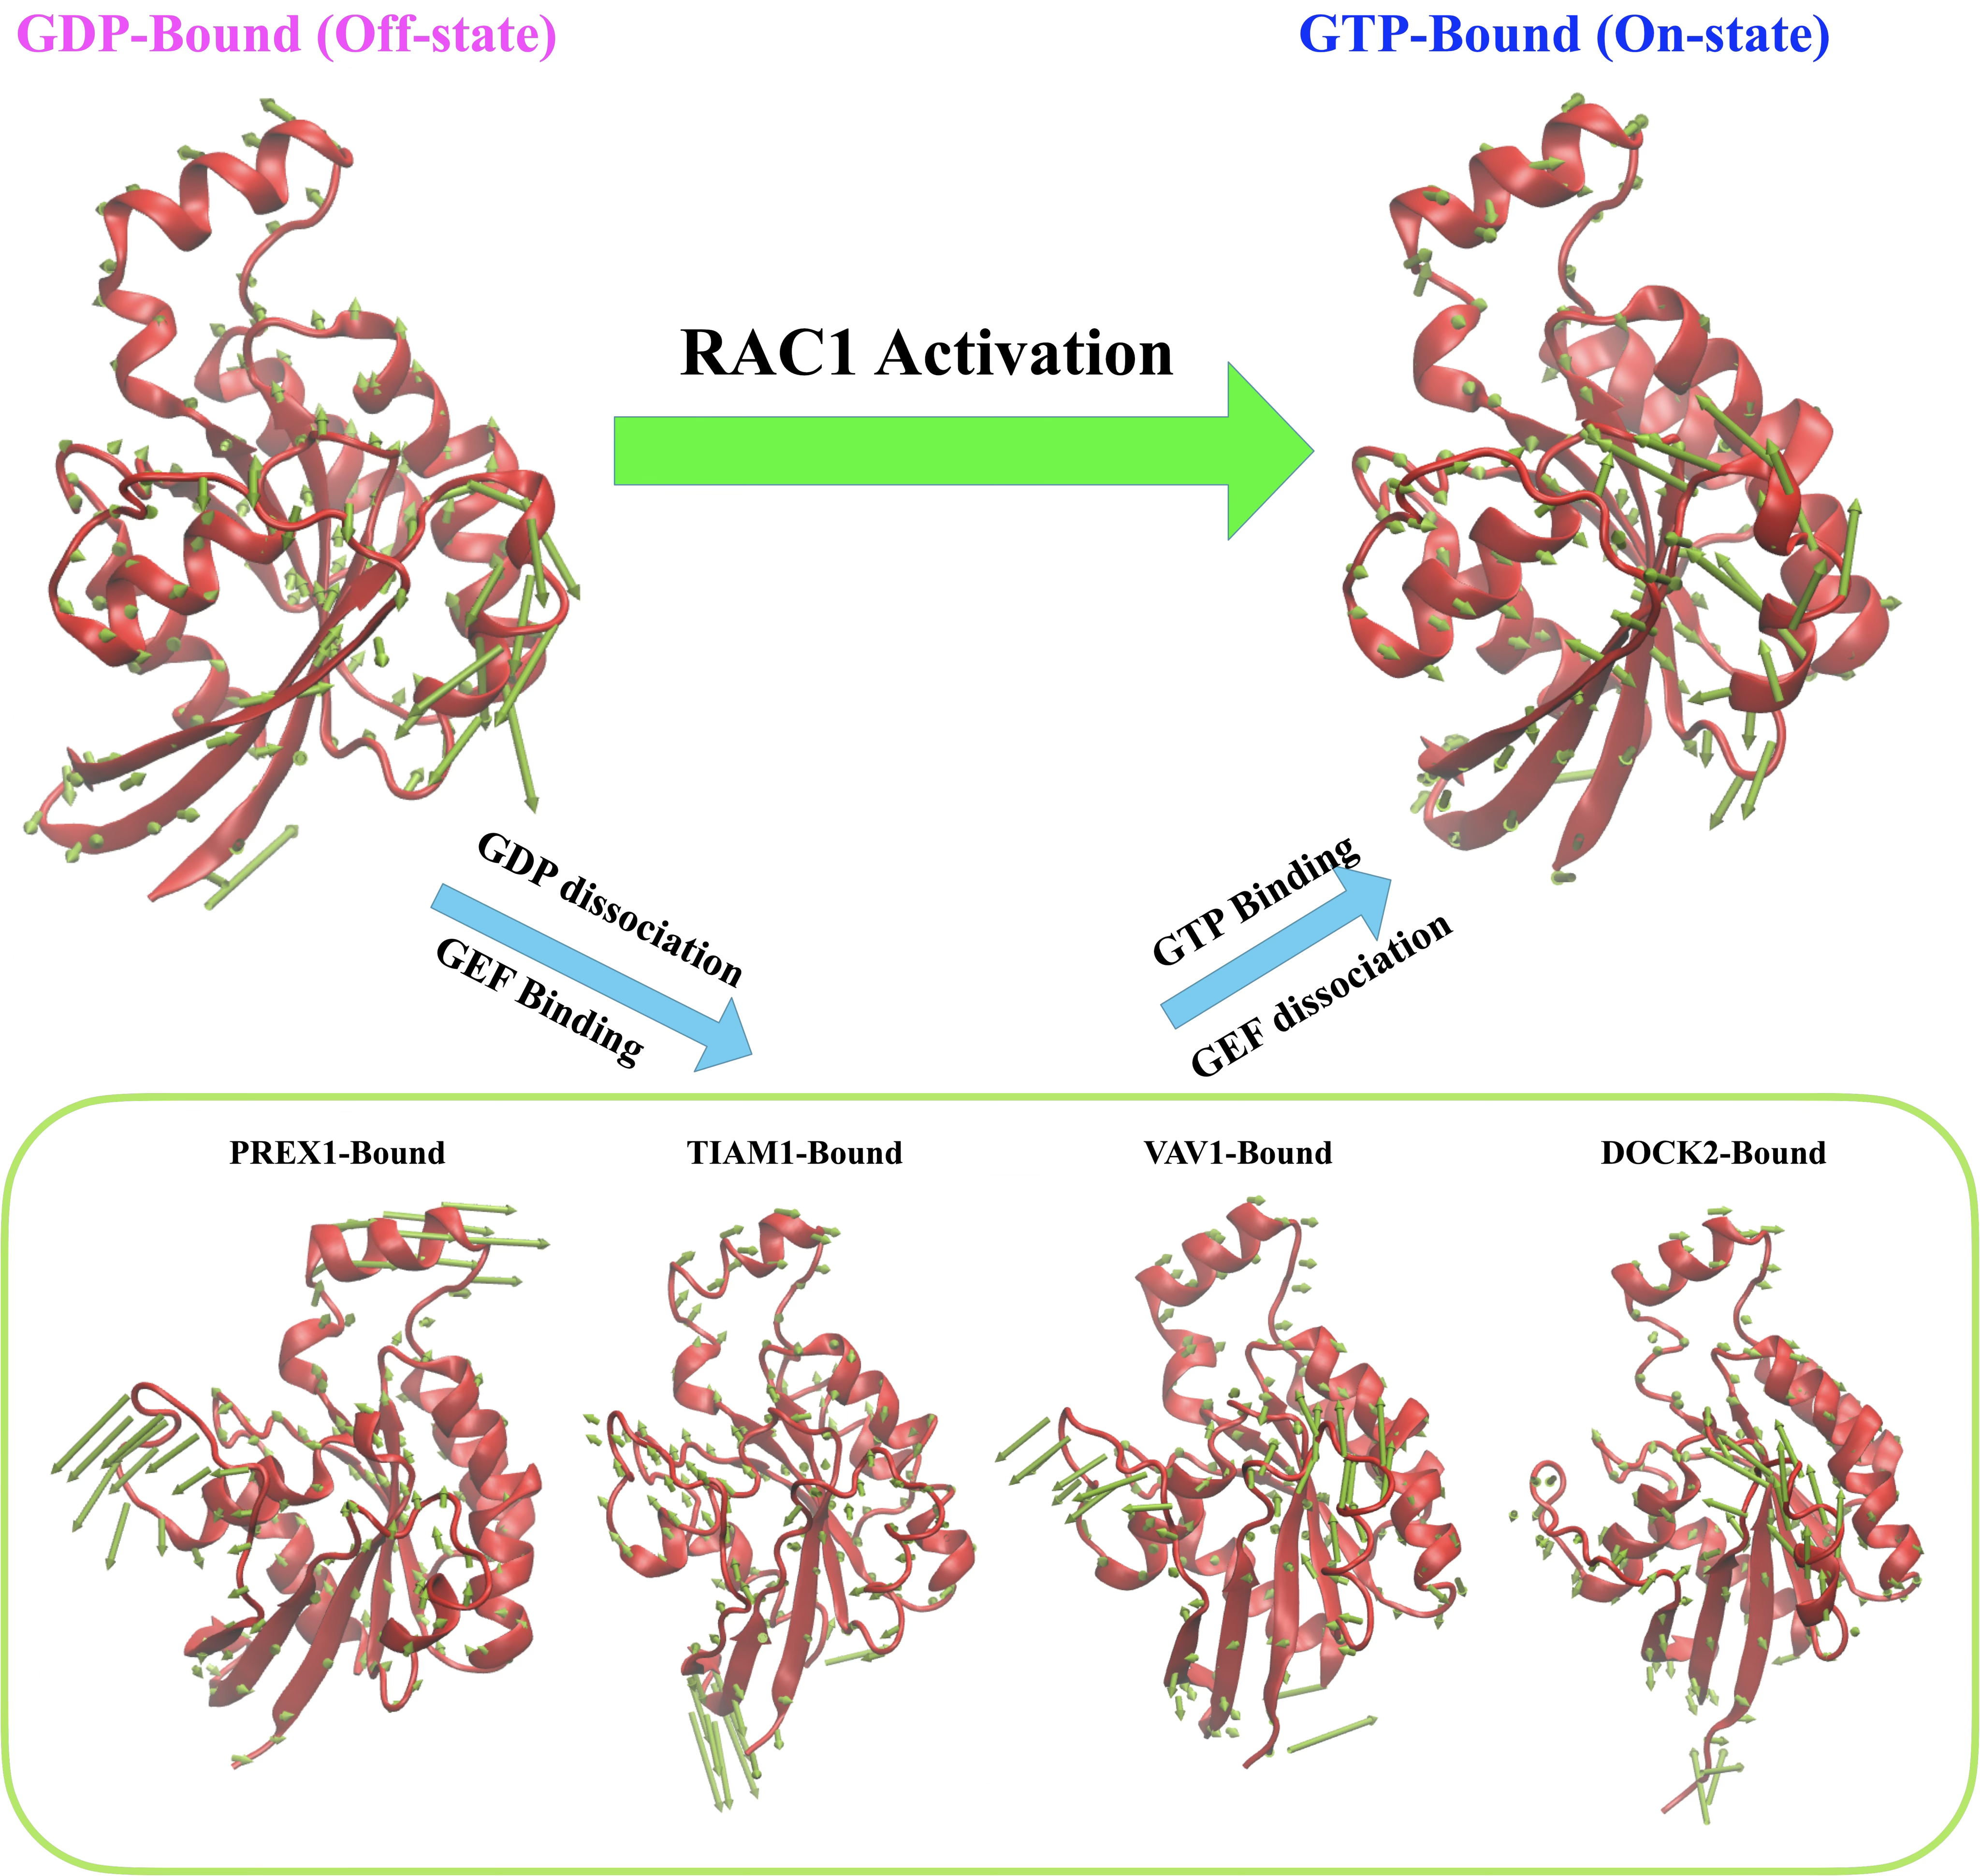
\includegraphics[width=1\textwidth]{PCA.jpg}
    \caption{Essential Dynamics of Rac1 protein to explain the opening and closing of the transient pockets induced by the \textcolor{red}{cosolvent molecular probes}. Magenta colour indicates the P-loop region. Orange colour indicates switch I region. Green colour indicates switch II region. Yellow colour indicates helical insert. IPA is isopropanol. \textbf{(A)} Projection of amplitude motions from PC1 on Rac1 structure. \textbf{(B)} Identification of Rac1 conformational clusters in various water and \textcolor{red}{cosolvent molecular probes} based on essential dynamics using PC1 and PC2.} 
    \label{fig:PCA}
\end{figure}

\textcolor{red}{In an attempt to identify the structural changes on the Rac1 surface that might explain the opening of the transient pockets, we extracted the essential dynamics using the principal component analysis of Rac1 following microsecond-scale cosolvent MD simulations. The purpose of such long time-scale simulations with and without \textcolor{red}{cosolvent molecular probes} is to evaluate the possibility of opening of the pockets, and to evaluate if an induced-fit mechanism is responsible for opening the pockets. The systems that were simulated without \textcolor{red}{cosolvent molecular probes} are treated as the reference systems for comparing the molecular probe-induced pocket opening.  In Rac1, like all other small G proteins, the switch regions show higher conformational flexibility. This flexibility is central to the switching mechanism for small G proteins that allows GEF and GAP binding, which is a prerequisite for nucleotide exchange and GTP hydrolysis, respectively.  The essential dynamics extracted from the dominant modes of motions by employing principal component analysis also confirm the large dynamical flexibility of the switch regions.  Therefore, we embarked on understanding if the switch region dynamics could play a role in the opening of these transient pockets. The essential dynamics for GTP and delGTP systems, simulated without cosolvent molecular probes, suggest that switch regions are the most dynamics region in the Rac1 protein (\textbf{Figure \ref{fig:PCA}A}). A significant ordering of switch I, and the P-loop is observed in the presence of GTP and Mg$^{2+}$ ion. This can be attributed to the strong electrostatic interactions shown by the phosphate group through the  Mg$^{2+}$ ion, which interacts with the switch I residues. The switch I loop was found exhibit largest flexibility in presence of the cosolvent molecular probes (\textbf{Figure \ref{fig:PCA}B}), especially by the aromatic probes. This could suggest that aromatic probes could destabilise the switch regions by increasing their conformational flexibility. However, we did not find a direct casual link between an increased flexibility of the switch regions and opening of the transient pockets. Furthermore, the dominant modes of motions suggested by PCA do strongly suggest that switch regions show highest conformational flexibility which is exploited by the GEF to regulate their activation state.}


\begin{figure}[hbt!]
    \centering
    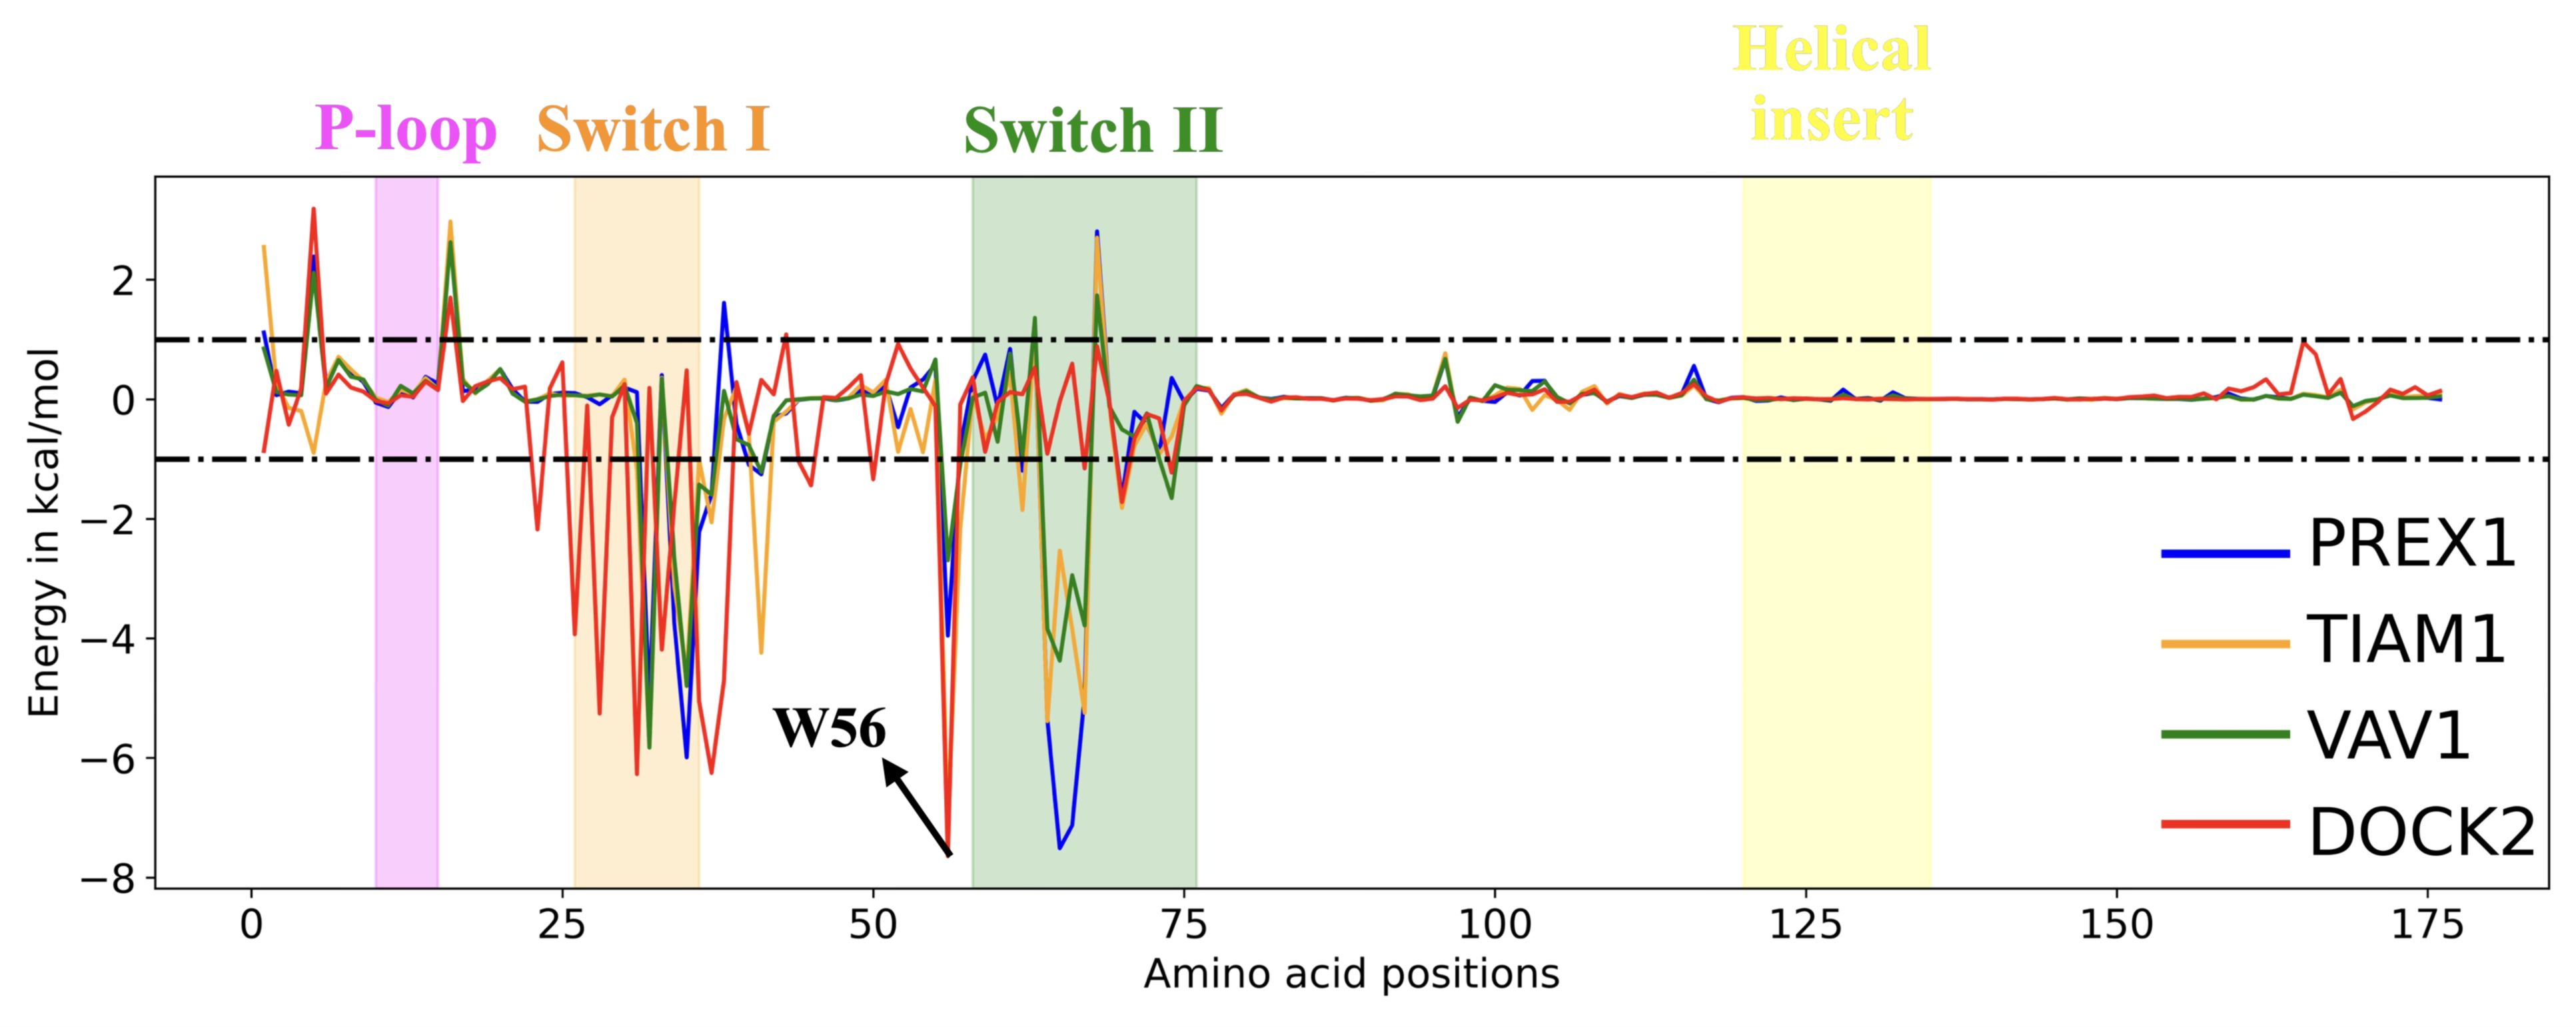
\includegraphics[width=1\textwidth]{mmgbsa_decomp.jpg}
    \caption{Per residue contribution to the effective binding affinity of the Rac1 residues to the GEFs as computed by MM/GBSA. The P-loop region is depicted in the magenta colour. The switch I region is depicted in orange, and the green coloured region is the switch II region. The helical region is shown in yellow. The residue W56 is marked due to its biological importance in the GEF binding. \textbf{(A)} Fluctuations of energetics contributions on the whole length Rac1. \textbf{(B)} Per residue contribution from site P1 residues. \textbf{(C)} Per residue contribution from site P2 residues. \textbf{(D)} Per residue contribution from Site P3 residues. \textbf{(E)} Per residue contribution from Site P4 residues. The dot-dash line indicates an arbitrary cutoff placed at \textbf{$\pm$1 kcal/mol}, which suggests that energy values outside this region contribute significantly to the binding of GEFs. } 
    \label{fig:decomp}
\end{figure}

So far, we have observed that most of the transient pockets in Rac1 open to accommodate the GEFs required for the nucleotide exchange. Hence, we found it prudent to analyse the energetic contribution of the Rac1 residues that are involved in GEF binding(\textbf{Figure \ref{fig:decomp}}). Furthermore, we attempt to locate how many amino acid residues important for GEF binding also make up the four transient sites, and thus, the per-residue contribution can indicate the binding hot spots for small molecules. As described earlier, there is a dominant role of the switch regions in GEF binding that leads to dissociation of GDP and association of GTP. This nucleotide exchange, catalysed by the GEF, necessitates their interaction with the switch regions, thus modulating their conformation such that it facilitates this exchange. The sites P1, P2 and P3 are located in the vicinity of the GEF binding region on Rac1(\textbf{Figure \ref{fig:decomp}B to \ref{fig:decomp}E}). A thorough analysis of the X-ray crystallographic structures suggests that important amino acid residues in Rac1 involved in GEF binding and activation are located in the switch I and II regions\cite{prex1pdb, tiam1pdb, vav1pdb, dock2pdb}.

\begin{figure}[hbt!]
    \centering
    \includegraphics[width=1\textwidth]{fig_transient_sites_withGEFs.jpg}
    \caption{Rac1-GEF complexes with four transient sites illustrated to understand the orientation of various GEFs on the Rac1 surface. Rac1 is shown in a grey surface representation. All GEFs are shown as a cartoon representation. The transient pockets are displayed in sphere representation: blue for site P1, cyan for site P2, magenta for site P3, and asparagus for site P4.} 
    \label{fig:site_gefs}
\end{figure}

Site P1 is located in the cavity that forms between switch I and II, which is the region where all the GEFs bind to perform their functions (\textbf{Figure \ref{fig:site_gefs}}). Seven residues (T35, V36, F37, D38, W56, and D57) lining this site contribute significantly to GEF as shown by MM/GBSA per residue decomposition. From the crystallographic data, the backbone amides of T35 and V36, which are located on the switch I region, show hydrogen bonding interactions with conserved GEF residues, such as E56(PREX1)\cite{prex1pdb} and E201(VAV1)\cite{vav1pdb}. F37 and D38, which are also located on the switch I region, show pronounced favourable interactions with DOCK2 residues (\textbf{Figure \ref{fig:decomp}B}). W56 is a key determinant of selectivity across both DOCK and DH-PH GEF families. In Rac1, W56 is a bulky residue that inserts into a pocket formed in the GEFs, and its presence generally supports activation by Rac-specific DOCKs. W56 is also the only residue that forms part of Site P1 and P2; therefore, designing small molecules that increase interaction with it could lead to competition with GEF binding. In summary, the residues that form Site P1 and P2 show a significant number of interactions with GEF proteins. Furthermore, we also observe in Figure \ref{fig:decomp} that there are residues that selectively bind to different GEFs that could be targeted for GEF-specific modulations. For example,  F37 and D38 show markedly greater interaction with DOCK2 than other GEFs used in this study; therefore, small. Molecules that show stronger interactions with these residues could selectively compete with the DOCK2 protein. In case of sites P3 and P4, residues interact with GEFs (\textbf{Figure \ref{fig:decomp}D} and \textbf{\ref{fig:decomp}E}). However, a few residues in site P3 show modest interaction with DOCK2, which makes this pocket more amenable to targeting and modulating Rac1-DOCK2 interaction (\textbf{Figure \ref{fig:site_gefs}}).

\section{Conclusion}
\textcolor{red}{The computer simulations reported in this work reveal that Rac1 harbours four transient. We tested the opening of these transient pockets using cosolvent molecular probes probes that suggest an induced-fit mechanism, revealing the transient nature of the pockets. Sites P1 and P2 are located in the regions that form the GEF docking interface, while sites P3 and P4 map to regions engaged by the DOCK-family of GEFs and the ELMO1 cofactor. Pocket-volume fluctuations across nucleotide- and GEF-bound states, measured by microsecond-scale MD simulations using redcosolvent molecular probes, demonstrate that several of these pockets cross the druggability threshold of the pocket volume. This behaviour confirms their transient nature and warrants an induced-fit mechanism that triggers the opening of the pockets. Taken together, these findings suggest that Rac1, which was considered undruggable, can in fact be modulated using small molecules that target the transient pocket identified in this work. We strongly believe that this work offers new opportunities to target specific Rac1 protein with small molecules.} 


\begin{acknowledgement}
This research was supported by a grant from Agence Nationale de la Recherche (ANR), grant number ANR-22-CE18-0015-03. This research used resources of the GLiCID Computing Facility (Ligerien Group for Intensive Distributed Computing, Pays de la Loire, France, https://doi.org/10.60487/glicid.). EM and ST extend their gratitude to Yves-Henri SANEJOUAND and Bernard OFFMANN (US2B, Nantes Université) for their suggestions to improve this work. 
\end{acknowledgement}

\section{Data and Software Availability}
All software tools used for this work are mentioned in the methods and listed in the references. All the software mentioned and used for this work can be obtained from the respective references. The files associated with this project can be downloaded freely from  \url{https://gitlab.univ-nantes.fr/martis-e/orbit_ambermd.git}

\begin{suppinfo}

\textcolor{red}{List of supplementary Tables}
\begin{itemize}
 \item \textcolor{red}{\textbf{Table \ref{SI-tbl:SI-Heating using NVT Ensemble}}: Details of stages of Heating using NVT Ensemble}.
 \item \textcolor{red}{\textbf{Table \ref{SI-tbl:SI-pocketParameters}}: Parameters used for pocket identification in POVME2}.
 \item \textcolor{red}{\textbf{Table \ref{SI-tbl:SI-Fpocket}}: Results of Pocket Detection using Fpocket.}
\end{itemize}

List of supplementary figures
\begin{itemize}
    \item \textbf{Figure \ref{SI-fig:SI_CORRNUC}}: Pearson's Correlation for the volume fluctuations among different pockets and the effect of nucleotide binding.
    \item \textbf{Figure \ref{SI-fig:SI_CORRGEF}}: Pearson's Correlation for the volume fluctuations among different pockets and the effect of GEF binding.
    \item \textbf{Figure \ref{SI-fig:SI_screeplot}}: Scree plot to compute the cumulative variance explained by principal components.
    \item \textbf{Figure \ref{SI-fig:SI_combinedpockets}}: Analysis of pocket volume changes by combining pockets P1 with P2, and P3 with P4.
    \item \textbf{Figure \ref{SI-fig:SI_RMSD_FL}}: Time-evolution of RMSD of backbone atoms from Full Rac1 protein.
    \item \textbf{Figure \ref{SI-fig:SI_RMSD_PL}}: Time-evolution of RMSD of backbone atoms from the P-loop region.
    \item \textbf{Figure \ref{SI-fig:SI_RMSD_S1}}: Time-evolution of RMSD of backbone atoms from the switch I region.
    \item \textbf{Figure \ref{SI-fig:SI_RMSD_S2}}: Time-evolution of RMSD of backbone atoms from the switch II region.
    \item \textcolor{red}{\textbf{Figure \ref{SI-fig:SI_P1_VOL}}: Time-evolution of pocket volume for Site P1}.
    \item \textcolor{red}{\textbf{Figure \ref{SI-fig:SI_P2_VOL}}: Time-evolution of pocket volume for Site P2}.
    \item \textcolor{red}{\textbf{Figure \ref{SI-fig:SI_P3_VOL}}: Time-evolution of pocket volume for Site P3.}
    \item \textcolor{red}{\textbf{Figure \ref{SI-fig:SI_P4_VOL}}: Time-evolution of pocket volume for Site P4.}
    \item \textcolor{red}{\textbf{Figure \ref{SI-fig:SI_RDF}}: Radial Distribution Function of the Molecular Probes computed for each of the new pockets identified in this work.}
    \item \textcolor{red}{\textbf{Figure \ref{SI-fig:SI_SASA_100ns}}: Analysis of the Solvent-Accessible Surface Area using a 1.4 \r{A} probe accross all the newly identified site to understand the effect of nucleotide and GEF binding.}
    \item \textcolor{red}{\textbf{Figure \ref{SI-fig:SI_SASA_cosolv}}: Analysis of the Solvent-Accessible Surface Area using a 1.4 \r{A} probe accross all the newly identified site to understand the effect of Molecular probes.}

\end{itemize}
\end{suppinfo}

\bibliography{references} 
\end{document}